\documentclass[dvips,letterpaper,12pt]{report}
\usepackage[square,numbers]{natbib}
\usepackage{url}
\usepackage{thesis}
\usepackage[dvips]{graphicx}
\usepackage{float}
\usepackage{caption}
\usepackage{subcaption}
%\usepackage{svg}
\usepackage{amsmath}
\usepackage{array}
\usepackage{mathtools}
\usepackage{multirow}
\usepackage{makeidx}
\usepackage{longtable}
\usepackage{listings}
\usepackage{color}
\usepackage{alltt}
%\usepackage{epstopdf}
%\numberwithin{equation}{section}

%\definecolor{dkgreen}{rgb}{0,0.6,0}
%\definecolor{gray}{rgb}{0.5,0.5,0.5}
%\definecolor{mauve}{rgb}{0.58,0,0.82}

\lstset{frame=tb,
  language=Java,
  aboveskip=3mm,
  belowskip=3mm,
  showstringspaces=false,
  columns=flexible,
  basicstyle={\small\ttfamily},
  numbers=none,
  numberstyle=\tiny\color{gray},
  keywordstyle=\color{blue},
  commentstyle=\color{dkgreen},
  stringstyle=\color{mauve},
  breaklines=true,
  breakatwhitespace=true
  tabsize=3
}
%\makeindex
\begin{document}

\pagenumbering{roman}

\thesistitle
	{A New Approach for Evaluation of Stereo Correspondence Solutions in Outdoor Applications of Augmented Reality}
	{Baharehsadat Pourazar}
	{Master of Sciences}
	{Department of Computer Science}
	{April 2014}

%\addcontentsline{toc}{chapter}{Abstract}
\begin{center}
\textbf{\large Abstract}
\end{center}
For many years, researchers have made great contributions in the fields of augmented reality (AR) and stereo vision. 
One of the most studied aspects of stereo vision since the 1980s has been \textit{Stereo Correspondence}, which is the problem of 
finding the corresponding pixels in stereo images, and therefore, building a disparity map.
As a result, many methods have been proposed and implemented in order to properly address this problem. 
Due to the emergence of different techniques to solve the problem of stereo correspondence, having an evaluation scheme to assess 
these solutions is essential. Over the past few years, different evaluation schemes have been proposed 
by researchers in the field to provide a testbed for assessment of the solutions based on specific criteria.
For instance, the Middlebury Stereo and the Kitti Stereo benchmarks
are two of the most popular and widely used evaluation systems through which a solution can be evaluated and compared 
to others. 
However, both of these models take a general approach towards evaluating the methods, that is, they 
have not been designed with an eye to the particular target application.
In our proposed approach, steps are taken towards an evaluation design based on the potential applications of stereo methods.
Considering the target application while evaluating the methods enables us to better define the criteria for \textit{efficiency}, that is, the processing time, 
and the required accuracy of the disparity results.
Since AR has attracted more attention in the past few years, 
the evaluation scheme proposed in this research is designed based on outdoor AR applications which take can advantage of
stereo vision techniques to obtain a depth map of the surrounding environment. This map can be used to
integrate virtual objects in the scene that respect the occlusion effects that are expected to occur based on the depth of the real objects. 


%\addcontentsline{toc}{chapter}{Acknowledgements}
\begin{center}
\textbf{\large Acknowledgements}
\end{center}

\vspace{1cm}

Foremost, I would like to express my sincere gratitude to my supervisor, Dr. Oscar Meruvia-Pastor, for his continuous support, motivation, and 
kind guidance throughout my research program. This 
thesis would have not been possible without the generous resources provided by him, the Department of Computer Science, and Memorial University.

I would like to express my heartfelt appreciation to Dr. Sam Bromley for his patience, constant encouragement, and insightful, challenging comments which compelled me to always
do better.

I am deeply grateful to my family who never stopped supporting me throughout all my studies, even when we were far from each other. I would have never been the person I am today if 
it was not for their unconditional support.

Last but not the least, I want to thank my fellow labmates in Computer Vision Lab for the interesting ideas we shared, for all the sleepless nights we spent together before deadlines, 
and for all the fun we had together in the last two years. Studying at Memorial University along with my peers in the department has been a great experience for me
and is absolutely an unforgettable memory.

\tableofcontents

\addcontentsline{toc}{chapter}{List of Figures}
\listoffigures



\pagenumbering{arabic}
\documentclass[dvips,letterpaper,12pt]{report}
\usepackage[square,numbers]{natbib}
\usepackage{url}
\usepackage{thesis}
\begin{document}
\chapter{Introduction}

Augmented reality (AR) systems combine standard video inputs with computer-generated objects and
usually provide real-time interaction for the users. Combining virtual objects and annotations with real
world scenes has proved to be an effective way of conveying information about the surrounding environment to
the user and can be useful in many applications such as gaming industry, medical surgeries, tourism and etc.

Many mobile augmented reality system prototypes have been built over the past decades, from touring machine in 1997 \cite{fei97} 
to google AR glasses which was announced in 2013 \cite{google}; however most of these prototypes remained as laboratory prototypes
due to certain difficulties and constraints of using them in practical applications. To name some of the most important constraints
we can refer to \cite{liv05}:
\begin{enumerate}
\item The requirement of having more advanced hardware and technology to implement the systems properly
\item Human factors in augmented reality
\item Providing real-time interaction between user and the system
\end{enumerate}

AR systems overlay 2D or 3D virtual objects over real scenes. Therefore, depending on the application usage, certain accuracy would be required for 
registeration of virtual and real objects. There are different approaches to obtain user's location and the position of other objects in the environment.
Tracking sensors such as gyroscope and accelerometer along with video sensors can provide information on the user's position and viewing orientation \cite{azum01}.
In order to find the position of the objects in the scene, a depth map of the surrounding environment at each time would be required. In order to obtain the depth of the 
objects in the scene several depth sensing technologies can be used such as 3D laser scanner, depth cameras or regular cameras. However, in order to have a mobile AR
system which should be easy to carry around, the weight of the whole system would be a concern, hence, 3D laser scanners and depth cameras are not good choices for such systems.
Depth cameras such as Kinect or DS325 have certain limitation in viewing range (1m-5m) which would get less and worse in outdoor environments. On the other hand, 3D laser scanners can
generate very accurate depth maps, but they are normally expensive and their price would range from 500\$ to 50,000\$. Therefore, among all these technologies, using several 
cameras to generate a depth map of the surrounding environment seems to be the most efficient approach for outdoor 3D mobile augmented reality systems. {\newline}
In computer vision there are certain techniques to find the depth of the objects in an environment using one or more stereo pairs taken from slightly different point of view of the same scene. 
This class of techniques is called {\it Stereo Correspondence} or {\it Stereo Matching} \cite{sze11}. Stereo matching is one of the most sutdied subjects in computer vision and there
are many solutions proposed by researchers to address this problem using different techniques; however, finding the corresponding pixels in stereo pairs with certain level of accuracy and in real-time
for practical applications still remains a challenging task. {\newline}

Our motivation in this research is to study the possibility and usability of combining stereo vision approaches with AR systems. The particular application scenario we are interested in for
our study is a 3D mobile augmented reality system in urban settings. In order to pursue our goal for this research project, we have designed and implemented a testbed for evaluation of
stereo matching solutions based on specific criteria which will be described in more details later on in this document.
In the system of our ineterst, the depth map generated from two or multiple camera views will be used as the depth source to find the position of objects in the scene when
overlaying virtual objects at different locations and depth levels in the real environment. For our research we decided to study the effect of using stereo vision in an AR 
system on two of the most important constraints mentioned above, which are {\it human factors issues} and {\it real-time interaction}. {\newline}
Human perception of depth can vary depending on the environment under different circumstances. Many studies have focused on the evaluation of human perception of depth within different
criteria. One of these areas of study is human perception of depth in augmented reality which has recently attracted more attention. These studies show that human perception of depth
is inversely proportional to the viewer's distance from the object \cite{kru10,swa07,jer05,liv05}. In \cite{swa07} some experiments are designed to study and evaluate the human
perception of depth for outdoor augmented reality application in urban settings. Since the scope of the problem they are interested in is similar to the initial problem domain we 
were motivated by in this research, we have set our criteria for the error in human peception of depth based on their published results and we will consider it as a reference for the 
evaluation of the depth results from stereo matching solutions. \newline
Providing real-time interaction in an AR system for the user requires the processing time and update rate of the whole system to keep up idealy with the standard video frame rate, between 24fps and 30fps. However, studies show that in practice to build a reasonable interactive augmented world the processing rate should not be less than half of the video frame rate {\bf NOTE: Search for more valid refence} \cite{spe}. \newline
Therefore, based on the two important difficulties mentioned previously, we have designed our test bed in a way which enables us to particularly focus on evaluation of the results 
based on these factors. However, there is an important and unique feature in our designs of the experiments which is the focus on certain regions rather than the whole image. 
We believe that in an outdoor augmented reality application there are certain regions in a scene which are more important to human sight and erroneous registeration of virtual and 
real object in those regions can be easily picked out by the users. Wrong results in these regions can result in poor performance of the system and possibly wrong interaction between 
the user and both virtual and real worlds. We have defined these regions to be depth edges in the scene that have been expanded few pixels from each side. 
We believe that depth edges which will normally include object boundaries as well are important depth cues for the user to perceive the depth of different objects in the scene. 
The reason we have extended the detected edges to some pixels on each side is to also address occlusion and depth discontinuity. Finding correct depth values in these regions 
can lead to more accurate combination of virtual and real objects in the scene and therefore a more reasonable augmented world from the user point of view to interact with. \newline

In this research work, using our designed test bed we have evaluated two stereo matching algorithms as samples. These two algorithms are:
\begin{enumerate}
\item Semi-global stereo matching and mutual information by Hirschmuller \cite{hir08}
\item On building an accurate stereo matching system on graphics hardware \cite{mei11}
\end{enumerate}

The first algorithm by Hirschmuller has been implemented as part of Open Source Computer Vision Library (OpenCV). Therefore, we have used Opencv implementation of it that is 
call SGBM in our system. On the other hand, there was no source code available for the second algorithm. Therefore, the solution we used is our own implementation of the solution.

We have used Kitti stereo training dataset as our input stereo scenes, since they are proper samples taken from outdoor scenes under different conditions and the ground truth depth map
is also provided for each stereo pairs.



\bibliographystyle{plain}
\bibliography{reference} 
\end{document}

\chapter{Background and Related Works}
\label{chap:Background}

In this chapter we review the relevant concepts to this study and introduce the techniques used during this research work.

\section{Stereo Vision}

Stereo vision is the concept of viewing a scene (object) in the real world from slightly different
viewpoints at the same time which results in stereo image pairs that are used by the human visual system or computer vision techniques to convey
depth in a scene. 

Using computer vision techniques, it is possible to extract depth information from stereo
images. This process is called {\it Stereo Matching} or {\it Stereo Correspondence} in computer vision,
which in fact leads to the construction of a
3D model of a scene from two or multiple views by finding corresponding pixels and therefore, their spatial displacement within various views of the same scene \cite{sze11}.

Corresponding pixels in stereo images are the ones that represent the same point in the real
world. As it will be seen shortly in more detail, the amount of horizontal motion of such pixels
in stereo pairs, which is referred to as {\it disparity}, is inversely proportional to the
distance from the observer, i.e., depth; however,  estimation of the exact depth of the points requires some
other information as well, such as the position, and the calibration data of the cameras that were used to take the pictures.
While the physical and geometrical approaches to this problem are well understood by researchers in the field, the process of finding the corresponding pixels correctly, 
yet efficiently, and measuring the disparity to generate a dense depth map still remains a challenging task. \newline

\section{Epipolar Geometry}
Understanding the fundamentals of the underlying geometry of stereo matching helps to better understand the principal idea behind all the methods designed to address this problem, 
thus facilitating the comprehension of 3D model reconstruction from stereo image pairs. Therefore, we will thoroughly describe the basic geometry of stereo matching in this section. \newline
If we consider two cameras that are looking at a particular scene from slightly different view points, 
a back projection of any point in the 3D space via rays passing through each camera centre,
${C}^{'}$ and ${C}^{"}$, would result in two distinct points on each image plane. For simplicity, we will refer to the point 
in space as $P$, and its projection on the first (left) and second (right) image planes,
as $P^{'}$ and ${P}^{"}$ respectively. \newline
As a result of $P$'s back projection on the image planes, an important property will emerge between the points and the camera centres, which is coplanarity of all these points. 
This plane, also referred to as {\it epipolar plane}, passes through $P^{'}$, $P^{"}$ and the camera centres, thus intersecting each image plane. 
It should be noted that this property, from which the consequent properties are derived, is the building block of stereo matching methods. 
Let us denote the specified plane by $S$ for further reference. 
Since $S$ passes through the camera centres, it clearly traverses the line 
that connects two camera centres. This line, which is known as the {\it baseline}, intersects each image plane at a point called the {\it epipole}; denoted by ${e}^{'}$ and ${e}^{"}$
in Figure \ref{fig:epg}. 
Consequently, the intersection of the plane $S$ and each of the image planes, creates a line called {\it epipolar line} \cite{hart2000}. 
The {\it epipolar line} always passes through the {\it epipole} in the image plane. 
These concepts, illustrated in Figure \ref{fig:epg}, constitute the important components of the stereo correspondence geometry.

\begin{figure}[!h]
\centering
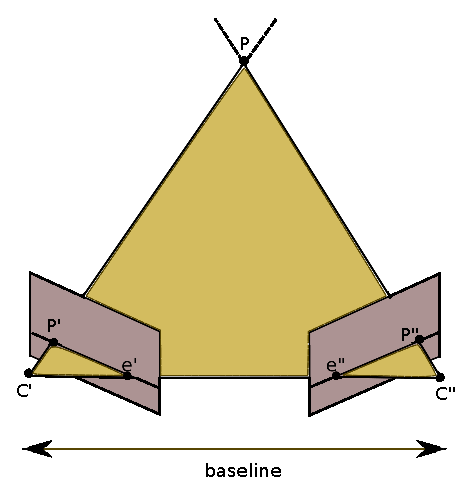
\includegraphics[width=0.5\textwidth]{epipole}
%\includesvg{epipole}
\caption{Epipolar geometry}
\label{fig:epg}
\end{figure} 

Now, we can define the problem of stereo correspondence as a case in which the location of $P^{'}$ in the image plane is known, while the
corresponding point $P^{"}$ is unknown; therefore, the problem can be stated as an attempt to find the correspondence of $P^{'}$ in the second image plane. Based on the aforementioned 
properties, we know that $P^{"}$ is located somewhere on the line, the epipolar line,
created by the intersection of the plane traversing the ray that goes through $P^{'}$ and the first camera centre and the {\it baseline}. This line is in fact, the projection of the ray going
through $P^{'}$ and the first camera centre, on the right image plane. Therefore, the search for the corresponding point, $P^{"}$, will be limited to merely scanning the corresponding 
epipolar line on the second image plane rather than the whole image.

%\begin{figure}{h!}
%\centering
%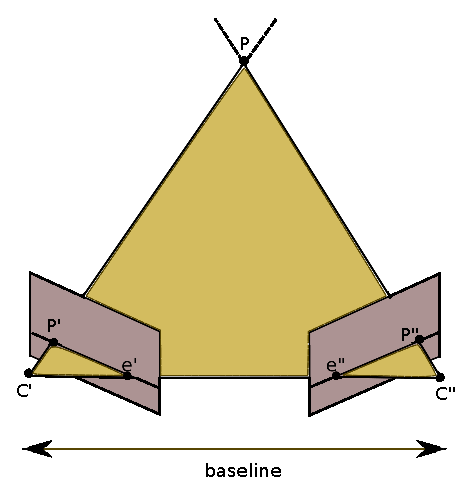
\includegraphics[width=1.5in,height=1.5in]{epipole}
%\end{figure}

It is now apparent that in order to find the correspondence of a particular point $P^{'}$, in the second image plane
the corresponding epipolar line, must first be sought. 
The projection from a point to its corresponding epipolar line can be obtained through certain transformations in space; normally a rotation and translation, Figure \ref{fig:rectify}.
For further geometrical calculations, these transformations can be represented
with a matrix that is only dependant on the camera's properties, not the scene \cite{hart2000}.
However, dealing with these transformations while looking for the corresponding points, can increase the complexity of stereo matching algorithms to certain levels \cite{sze11}; therefore, 
in order to avoid this issue, many stereo matching approaches are proposed based on the assumption that image pairs are first warped \cite{sze11}.
This process is known as {\it image rectification} which is basically achieved by first having the cameras rotated in a way that their optical axis, 
the line passing through the camera centre which is perpendicular to the image plane, are parallel to each other; 
that is their optical axis is perpendicular to the baseline. As a result of this transformation, the epipoles are sent to infinity. 
Furthermore, it might be necessary to have the cameras tilted so that their {\it y} axis also becomes perpendicular to the optical axis. 
After these two steps, corresponding epipolar lines actually become horizontal scanlines; Figure \ref{fig:rectify}. This pre-processing step significantly constrains the process of searching 
for corresponding points and eliminates certain complications in stereo matching algorithms \cite{sze11}.

\begin{figure}[!h]
\centering
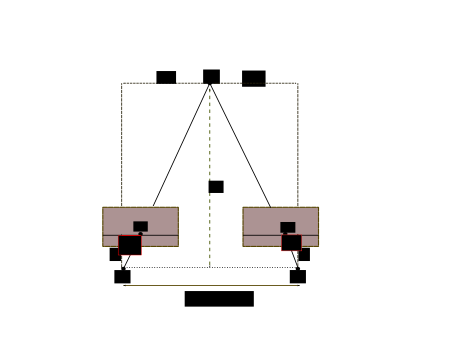
\includegraphics[width=0.65\textwidth,trim=22mm 0mm 0mm 150mm,clip]{rectdisp}
\caption{Rectified image pairs and disparity geometry}
\label{fig:rectify}
\end{figure} 

Sample stereo images taken using two regular webcams are displayed in figures \ref{fig:unrect} and \ref{fig:rect},
before and after rectification. 
The red line shows how features get aligned in the left and right image after the rectification process.

\begin{figure}[h!]
\centering
\subcaptionbox{Left image unrectified}
[.5\linewidth]{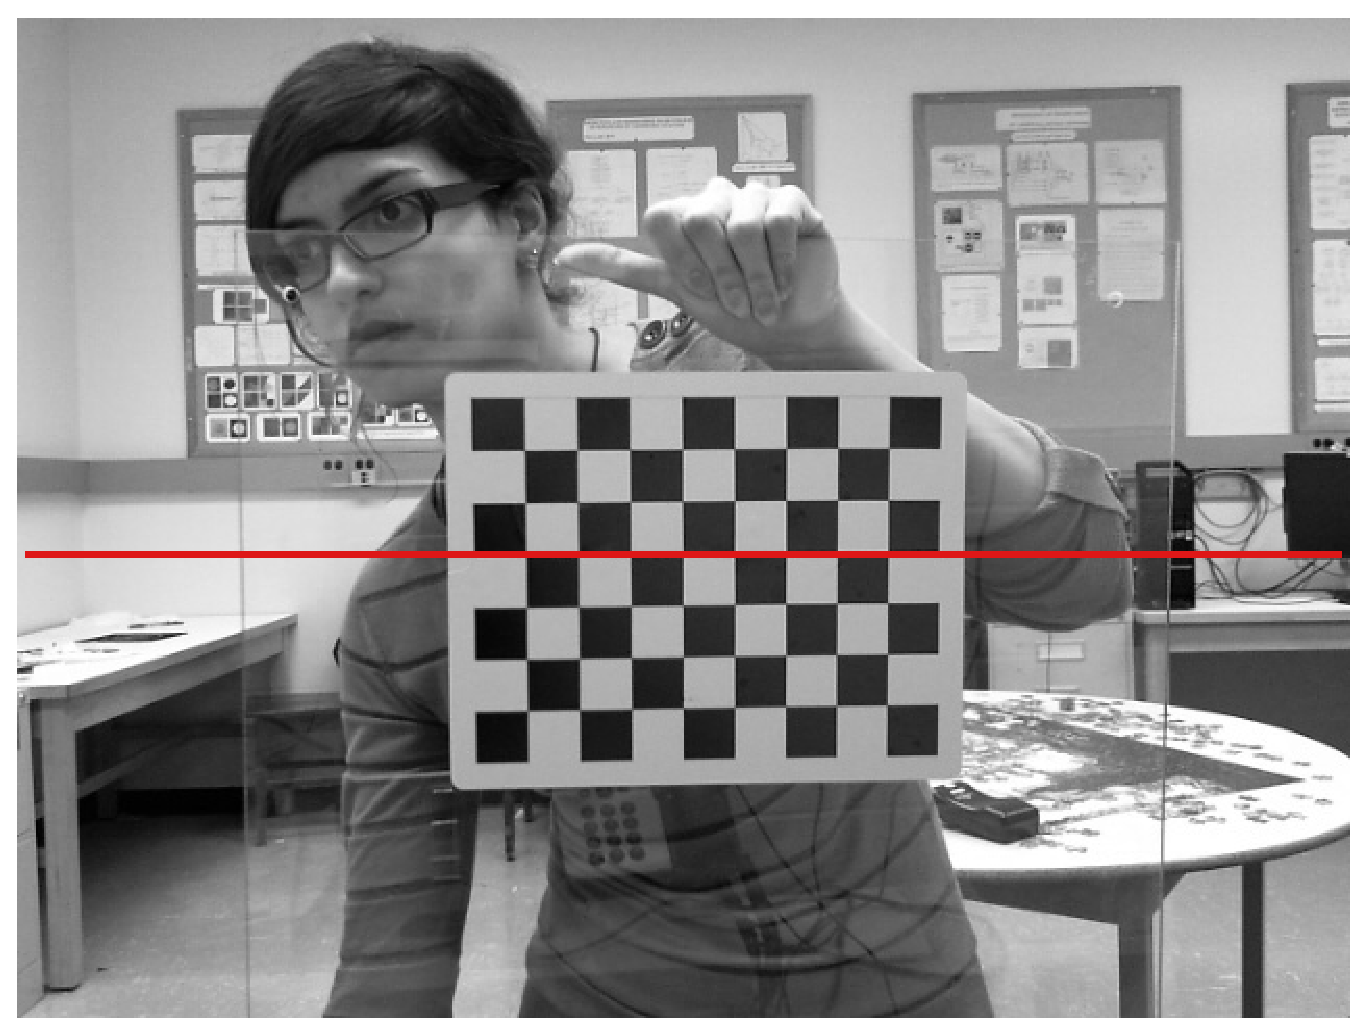
\includegraphics[scale=0.35]{RectL}}%
\subcaptionbox{Right image unrectified}
[.5\linewidth]{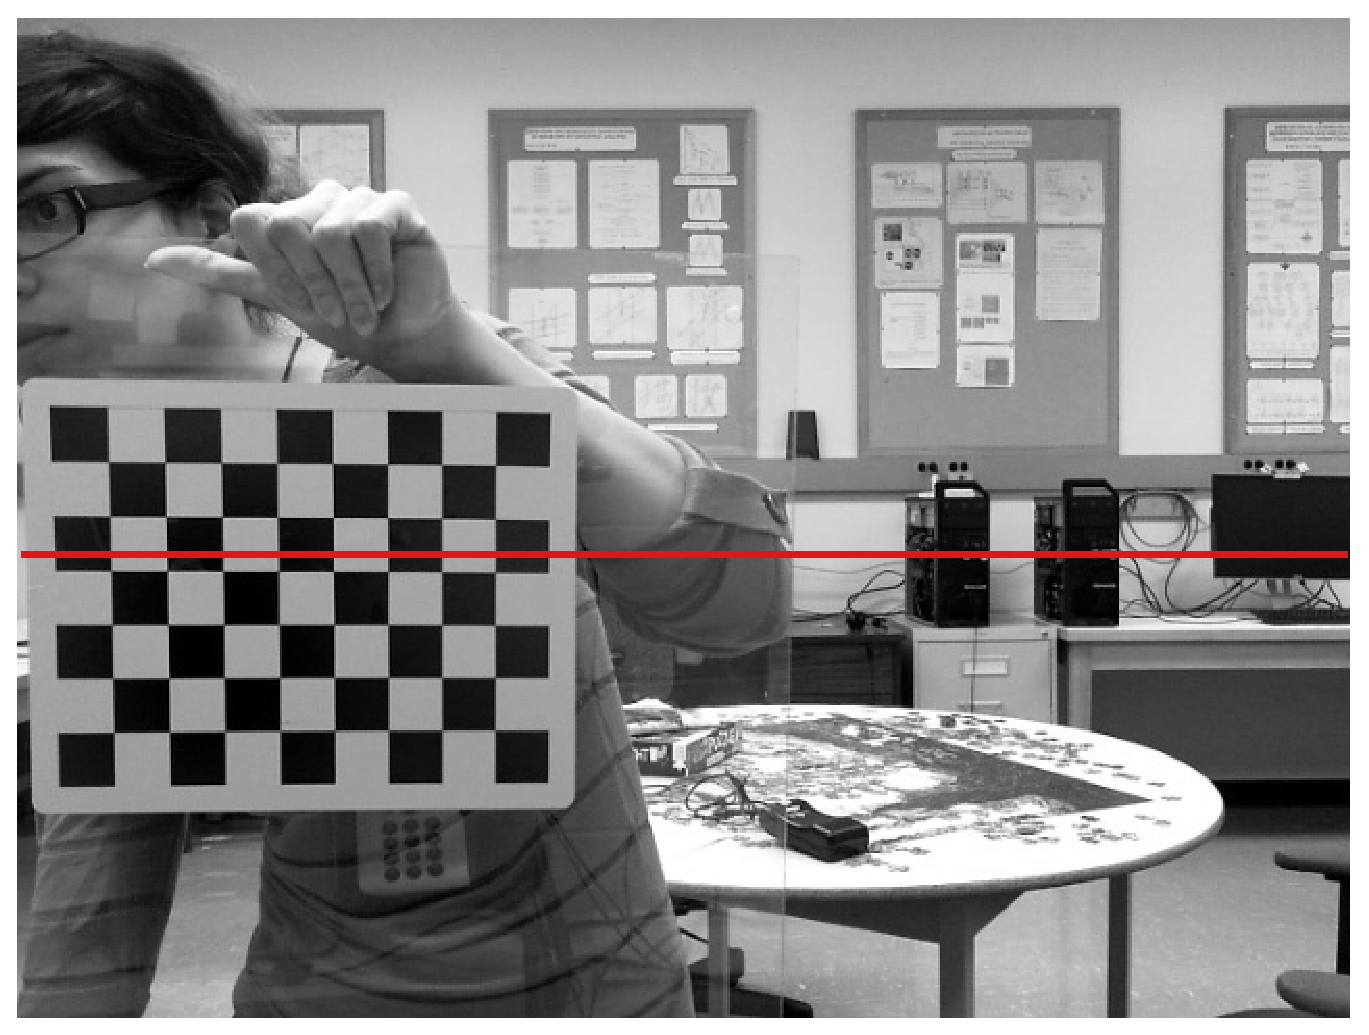
\includegraphics[scale=0.35]{RectR}}%
\caption{Sample stereo image before rectification}
\label{fig:unrect}
\end{figure}

\begin{figure}[h!]
\centering
\subcaptionbox{Left image rectified}
[.5\linewidth]{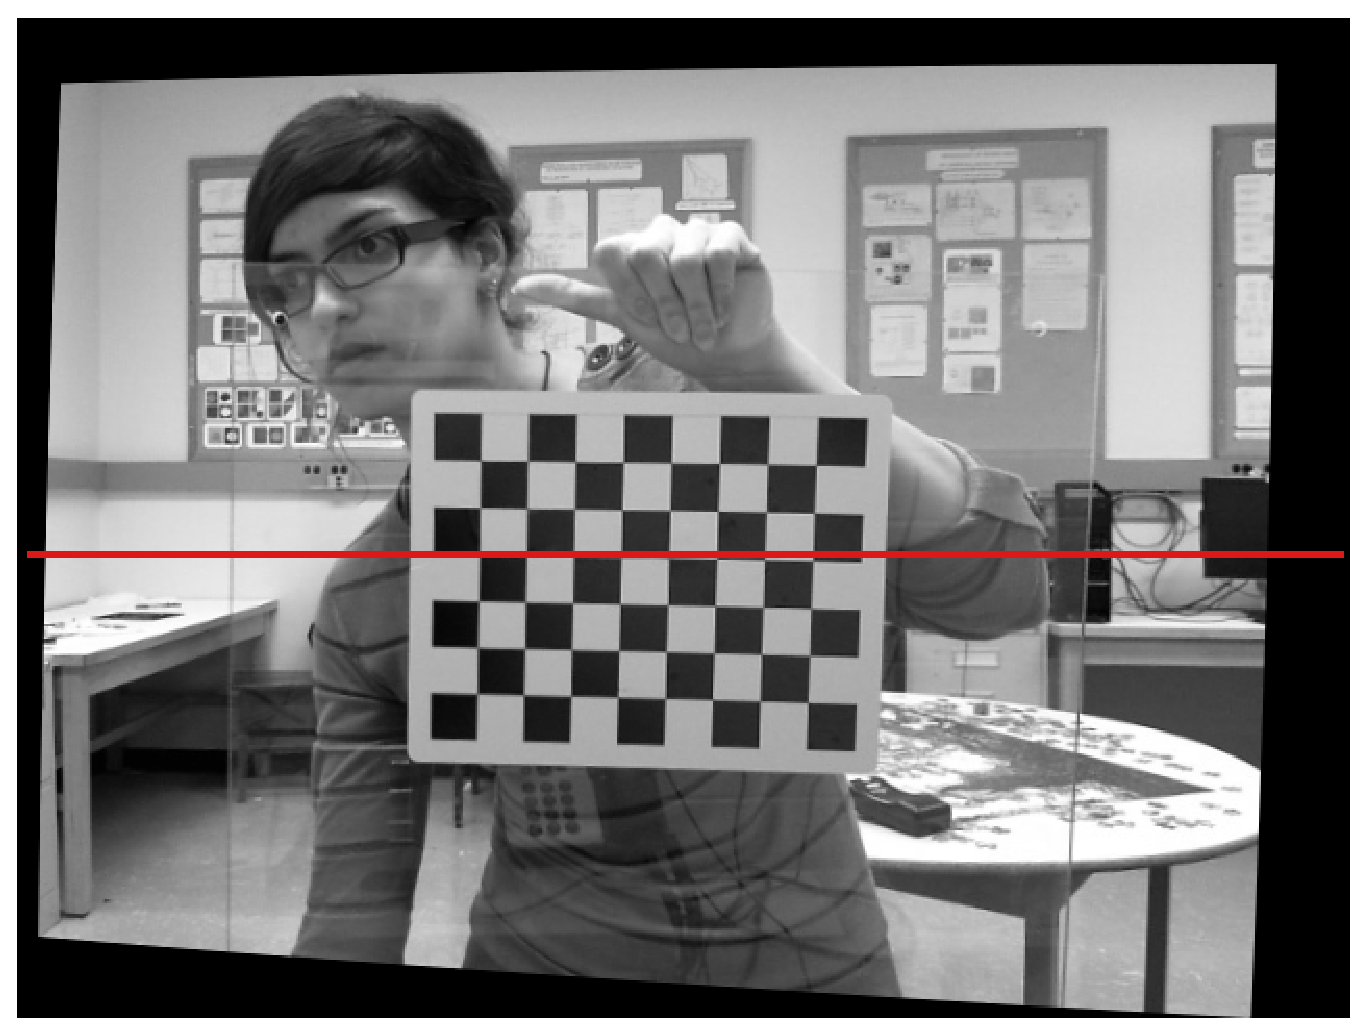
\includegraphics[scale=0.35]{rectLmark}}%
\subcaptionbox{Right image rectified}
[.5\linewidth]{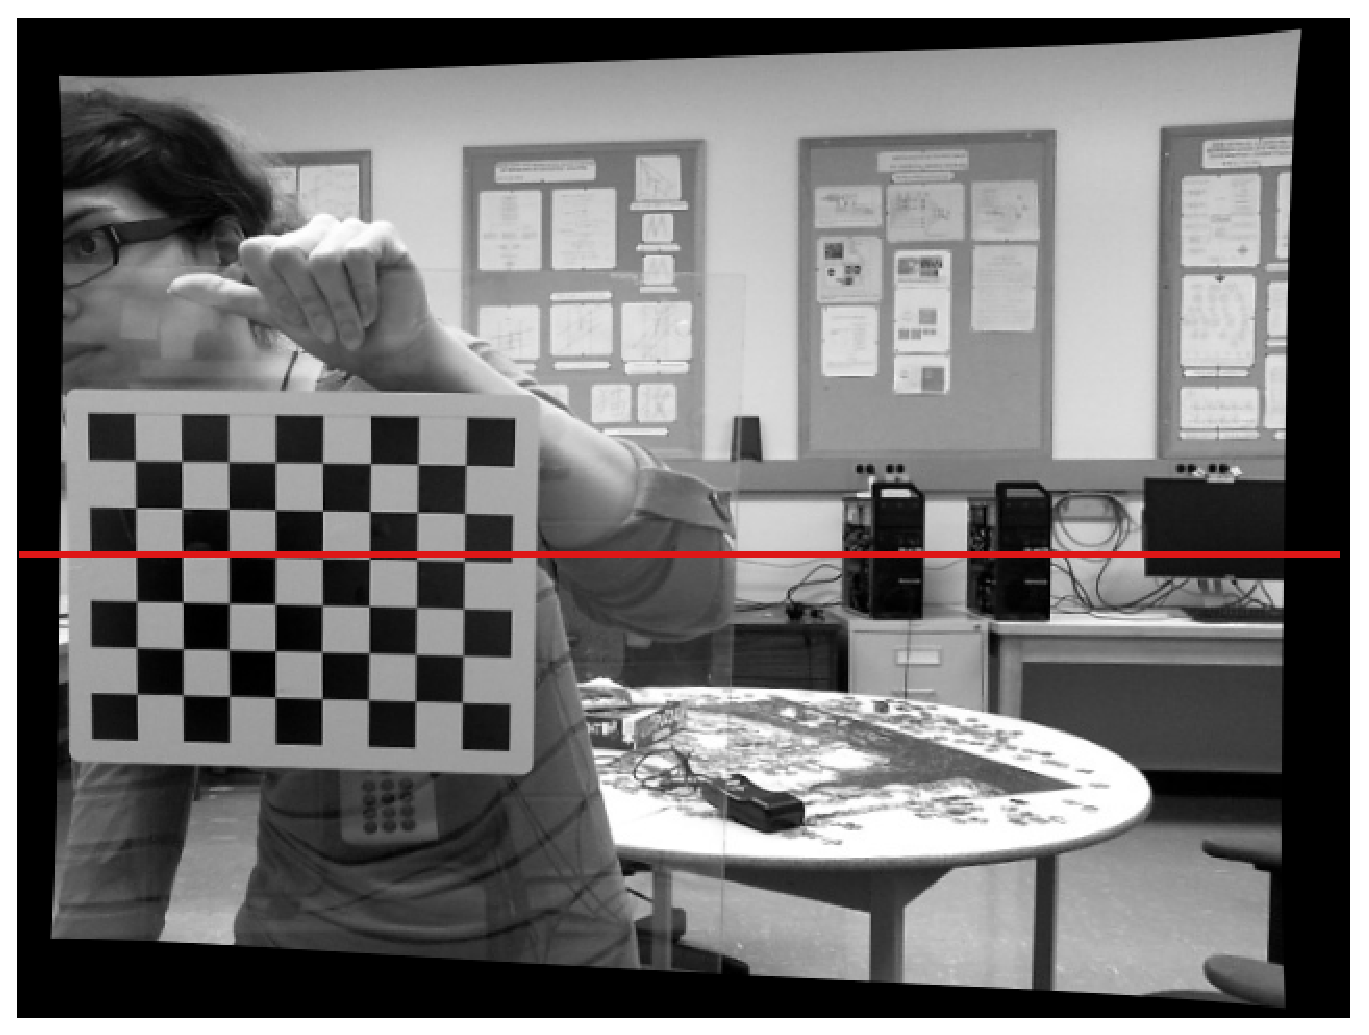
\includegraphics[scale=0.35]{rectRmark}}%
\caption{Sample stereo image after rectification}
\label{fig:rect}
\end{figure}

Using the rectification model and epipolar geometry described earlier, 
derivation of the geometrical relation through which the depth of a certain point in 3D space 
can be obtained, will be straightforward. This relation is presented as follows \cite{sze11}:
\begin{align}
\frac{X_{L}}{Z} &= \frac{x_{l}}{f} \label{eq:1} \\
\frac{-X_{R}}{Z} &= -\frac{x_{r}}{f}  \Rightarrow B-\frac{X_{L}}{Z}=-\frac{x_{r}}{f} \label{eq:2} \\
(\ref{eq:1}) + (\ref{eq:2}) \Longrightarrow  \frac{B}{Z} &= \frac{x_{l}-x_{r}}{f} \label{eq:3} \\
\intertext{if $x_{l}-x_{r}=d$, we will have:}
d &= \frac{Bf}{Z} \label{eq:dispeq}
\end{align}
where f is the {\it focal length} measured in pixels, B is the {\it baseline}, Z is the {\it 3D depth}, and d is the {\it disparity}. The relationship between corresponding pixels in the left
and right images according to disparity {\it d} is also as follows:
\begin{align}
{P}^{"}_{x} &= {P}^{'}_{x}+d(x,y) \\
{P}^{"}_{y} &= {P}^{'}_{y}
\end{align}
Therefore, based on the aforementioned formulas, the depth of points in 3D space can be easily calculated after finding the corresponding pixels in multiple views and consequently their
disparities \cite{bol87,oku93,sch02}.

\section{Stereo Correspondence Algorithms}
A survey of the field shows that the algorithms which address stereo correspondence problem can be roughly divided into two main classes \cite{sch02}. These classifications are commonly known as:
\begin{enumerate}
\item Sparse Correspondence Algorithms
\item Dense Correspondence Algorithms 
\end{enumerate}

Regardless of the category, stereo matching algorithms normally include specific steps in the process of finding the corresponding pixels in the stereo images.
According to the taxonomy by Scharstein et al. these steps are as followed:

\begin{enumerate}
\item {Calculation of matching cost}
\item {Aggregating the costs}
\item {Disparity computation}
\item {Disparity refinement}
\end{enumerate}

Depending on each algorithm, these steps and their sequence may change.

In this section, we are going to briefly describe the important specifications of the algorithms belonging to each of these two categories.
\subsection{Sparse Correspondence Algorithms}
Sparse correspondence algorithms, also known as feature-based algorithms, are the early stereo matching methods. In the 1980s, this class of algorithms received considerable attention by
many researchers in computer vision \cite{dhon89}.
In this type of methods, particular features in an image, such as edges, 
points, line segments, or other distinctive features are extracted; therefore, the search for corresponding pixels is only applied to these regions. 
Consequently, algorithms of this
sort result in a sparse disparity map \cite{matt89,hsie92, sze11}. The introduction of feature-based algorithms has mainly been motivated by three important factors \cite{bro03,sze11}:
\begin{itemize}
\item Lack of advanced hardware and technology for exhaustive computational tasks.
\item Constraint of the search area in order to find more reliable matches.
\item Stability of particular features to look for correspondences under certain circumstances where the image pairs are affected by external factors, 
such as illumination variations; in other words, when there is a considerable difference in photometric properties between the images pairs, 
particular features such as the edges may be more reliable to start the correspondence search.
\end{itemize}

However, the requirement of having dense depth maps for many applications and also the emergence of efficient {\it dense correspondence algorithms}, have diverted the attention away
from this class of algorithms in the last 20 years.

\subsection{Dense Correspondence Algorithms}
Unlike feature-based methods, dense correspondence algorithms try to find the
correspondences for all the pixels in the image, and therefore, result in a dense disparity map. Most recent algorithms and studies have focused on this class of algorithms since many applications 
nowadays, such as graphical rendering, 3D model construction, or augmented reality require a dense depth map of the scene. 
However, these algorithms face many challenges that need to be properly
addressed, such as finding the depth values in occluded regions, depth discontinuities, and textureless areas \cite{sch02,bro03}.

Dense correspondence algorithms are usually classified in two groups based on how they assign
disparities to pixels \cite{sze11}:
\begin{enumerate}
\item Local approaches
\item Global approaches
\end{enumerate}

\subsubsection{Local Approaches} 

Local methods tend to find the disparity of each pixel based on its neighboring pixels. In
other words, the disparity of a pixel is calculated in a finite window containing its neighboring pixels, based on a particular metric, e.g. the intensity values \cite{sch02}.

These methods make an implicit smoothness assumption for the pixels in the search
window, and therefore, assign the same disparity to all the pixels belonging to the same window which could result in incorrect disparity values in slanted surfaces or
depth discontinuities \cite{hirsch02}. This assumption can be considered as one of the major drawbacks of local methods.
Another drawback of local methods is their dependency on the window size \cite{sch02}. A fixed window size can raise certain problems in these algorithms:
\begin{enumerate}
\item If too large of a window size is considered, due to aforementioned smoothness assumption, the algorithm may result in blurry object boundaries and inaccuracy near depth discontinuities.
\item If the selected window size is too small, the disparity values will be less accurate and harder to find since little information has been considered for 
finding the correspondences of pixels in the image.
\end{enumerate}

However, a significant advantage of using local approaches is their high speed in finding disparity results.\newline

\subsubsection{Global Approaches}
Unlike local approaches, in global methods the disparity of a pixel depends on the information in
the whole image. Global methods usually include an optimization step of a global energy
function\cite{roy98,bobi99,boyk01,hong10}. In this class of algorithms, an optimal disparity value for each pixel is sought that leads to minimization of a global cost
function that normally combines a data term with an explicit smoothness assumption.

\begin{equation}
E(d)=E_{data}(d)+\lambda E_{smooth}(d)
\end{equation}
The term $E_{data}$ is normally defined as the difference of a common metric, e.g. the photometric property, between the corresponding pixels and is denoted as follows:

\begin{equation}
E_{data}(d) = \sum_{(x,y)}C(x,y,d(x,y))
\end{equation}

where C is a matching cost. The matching cost function can have various definitions depending on the algorithm; however, as mentioned above, it is normally defined as sum of absolute difference 
between the intensity of the corresponding pixels in two images \cite{sch02}.

The term, $E_{smooth}$, is the smoothness assumption based on which the disparity values in different regions are refined. The definition of this term can also vary in 
different solutions. $\lambda$ is also a weighting factor, by which the effect of the smoothness assumption in the global function can be controlled in the algorithm \cite{sze11}.
In order to find the minimum of the global function, certain approaches in computer science have proved to be particularly useful. 
To name some of these approaches, we can refer to dynamic programming \cite{kim05}, graph cut \cite{boy01,boyk01,boy04}, and belief propagation \cite{sun11}. 
Many researchers have studied and addressed the problem of stereo matching
by applying one of these approaches.

The major drawback of global approaches is normally their high usage of computational resources and low speed. However, 
they usually result in more accurate disparity values \cite{hirsch02,sze11}. 

It is also worthwhile to mention that in the past twelve years, another group of algorithms have emerged which cannot be explicitly classified in any of the previously mentioned groups.
These methods, which are known as {\it Segmentation-based techniques}, first segment the image into regions and then, rather than searching for correspondences per pixel,
they attempt to find the corresponding disparity for each region. A more detailed review of these methods can be found in chapter 11 of \cite{sze11}.

\section{Edge Detection}

As mentioned earlier in the ``Introduction'', salient {\it edges} in the scene are one of the important features 
that can be used in many applications, such as object detection, image stitching, or 3D model reconstruction.
Due to their importance and application in this research, we review some of the relevant concepts and techniques in computer vision in this section.

\subsection{Edges}
When looking at a scene, an edge is defined whenever the visual system can perceive a distinguishable variation in color, intensity or texture between 
different regions \cite{sze11}.
Therefore, a reasonable mathematical approach to detect the edges in an image would be calculating the gradient of the intensity image. However, since an image normally contains a certain amount of
noise which intensifies at higher frequencies, taking the derivatives of the image can lead to significant noise amplification, as it makes high frequency signals more prominent to others.
Therefore, it is better to attenuate high frequencies prior to applying any edge detection approach. 
There are a variety of filters for image smoothing (blurring); however, since we want to attenuate high frequencies, it is better to use a low-pass filter, which only passes low frequencies.
A widely known class of image blurring filters in computer vision are called {\it linear filters}, whose output is a linear function of their input. 
In linear filtering operators, for each pixel a weighted summation of its neighboring pixels
is used in order to estimate its final value \cite{sze11}. In mathematics, this process can be modelled by convolution of the input signal with a particular function, known as kernel. 
\begin{equation}
g(i,j)=\sum_{k,l}f(i+k,j+l)h(k,l)
\end{equation}
which is denoted as:
\begin{equation}
g=f\bigotimes h
\end{equation}
where $f$ and $g$ are the input and output signals respectively, and $h$ is the kernel function which can vary depending on the type of filter. 

Therefore, each filter can modify the input signal differently based on its corresponding kernel function.
The Gaussian filter is a filter commonly used for attenuating higher frequencies in an image and filtering out the noise \cite{wells86}. 
Since edges in an image may be oriented along any arbitrary direction, 
applying a filter which is biased towards a particular direction in filtering out the noise, would not be a prudent decision. Instead, a better choice would be choosing a filter 
with a symmetric 2D kernel function. 
This feature is particularly found in the Gaussian filter, since it employs a 2D symmetric kernel. Because of this unique feature, 
the Gaussian filter is normally used in most edge detection algorithms as a pre-processing step.
An isotropic, i.e. circularly symmetric, the Gaussian kernel has the following form \cite{sze11}:
\begin{equation}
G(x,y)=\frac{1}{2\pi \sigma ^{2}} e^{-\frac{x^{2}+y^{2}}{2\sigma^{2}}}
\end{equation}
where $\sigma$ is the standard deviation. 
A more thorough description of the Gaussian and some other types of filters can be found in chapter 3 of \cite{sze11}.

After smoothing the image with the Gaussian filter, the gradient of the smoothed image should be taken in order to detect the edges. This can be done by convolving 
the signal with a pair of convolution masks in each direction in order to detect the edges, both horizontally and vertically. An edge extracting operator called {\it Sobel} is normally used
for this purpose \cite{sze11}. 
Sobel convolution kernels for both x and y directions are defined as follows \cite{sze11}:

\begin{align}
G_{x} &= \begin{bmatrix}
-1 & 0 & +1 \\ 
-2 & 0 & +2 \\ 
-1 & 0 & +1
\end{bmatrix} \\
G_{y} &= \begin{bmatrix}
-1 & -2 & -1 \\ 
0 & 0 & 0 \\ 
+1 & +2 & +1
\end{bmatrix}
\end{align}

Following the estimation of image gradients in each direction, the magnitude and the direction of an edge element can then be found by \cite{sze11}:
\begin{align}
\left | G \right | &= \sqrt{G_{x}^{2} + G_{y}^{2}} \\
\theta &= \arctan (\frac{G_{y}}{G_{x}})
\end{align}

The process of applying the Sobel operator mask \cite{sobel78} to the smoothed image, is in fact equivalent to getting the first or second order directional derivative of the smoothed image 
and then look for zero crossings, i.e. where the sign of
the function changes \cite{sze11}. As a result of this process, edge elements are detected throughout the image.
After finding the edge points, it is desirable to have them linked to form continuous contours. Since adjacent edge elements are connected to each other, this can be easily achieved by linking
a detected edge element with its neighbors in both directions \cite{sze11}. As a result, a continuous chain of edges can be detected in the image.
The {\it Canny} edge detector, proposed by John F. Canny in 1986 \cite{canny86}, is one of the most commonly used edge detection approaches; however, it should be mentioned that in addition 
to the process described above for detecting the edges in the image, there are also two different thresholds defined 
in this approach that affect the edge linkage step. The purpose of having these two thresholds is elimination of streaks, i.e. certain breakage, that may appear along edge contours. 
By employing these thresholds in the process of edge detection and linkage, any value above the higher threshold will be output as an edge element and when linking the edge element 
to its neighbor to form a continuous contour, only those 
values above the lower threshold will be accepted \cite{canny86}. 
This process has shown to reduce the streaking effect to a significant amount \cite{canny86}. \newline
Figure \ref{fig:edgenodil} shows the detected edges obtained by applying the canny operation on the image \ref{fig:imggt5}.

\begin{figure}[H]
\centering

\includegraphics[scale=0.35]{imggt5}
\caption{Canny edge detection in an image}
\label{fig:imggt5}
\end{figure} 

\begin{figure}[H]
\centering
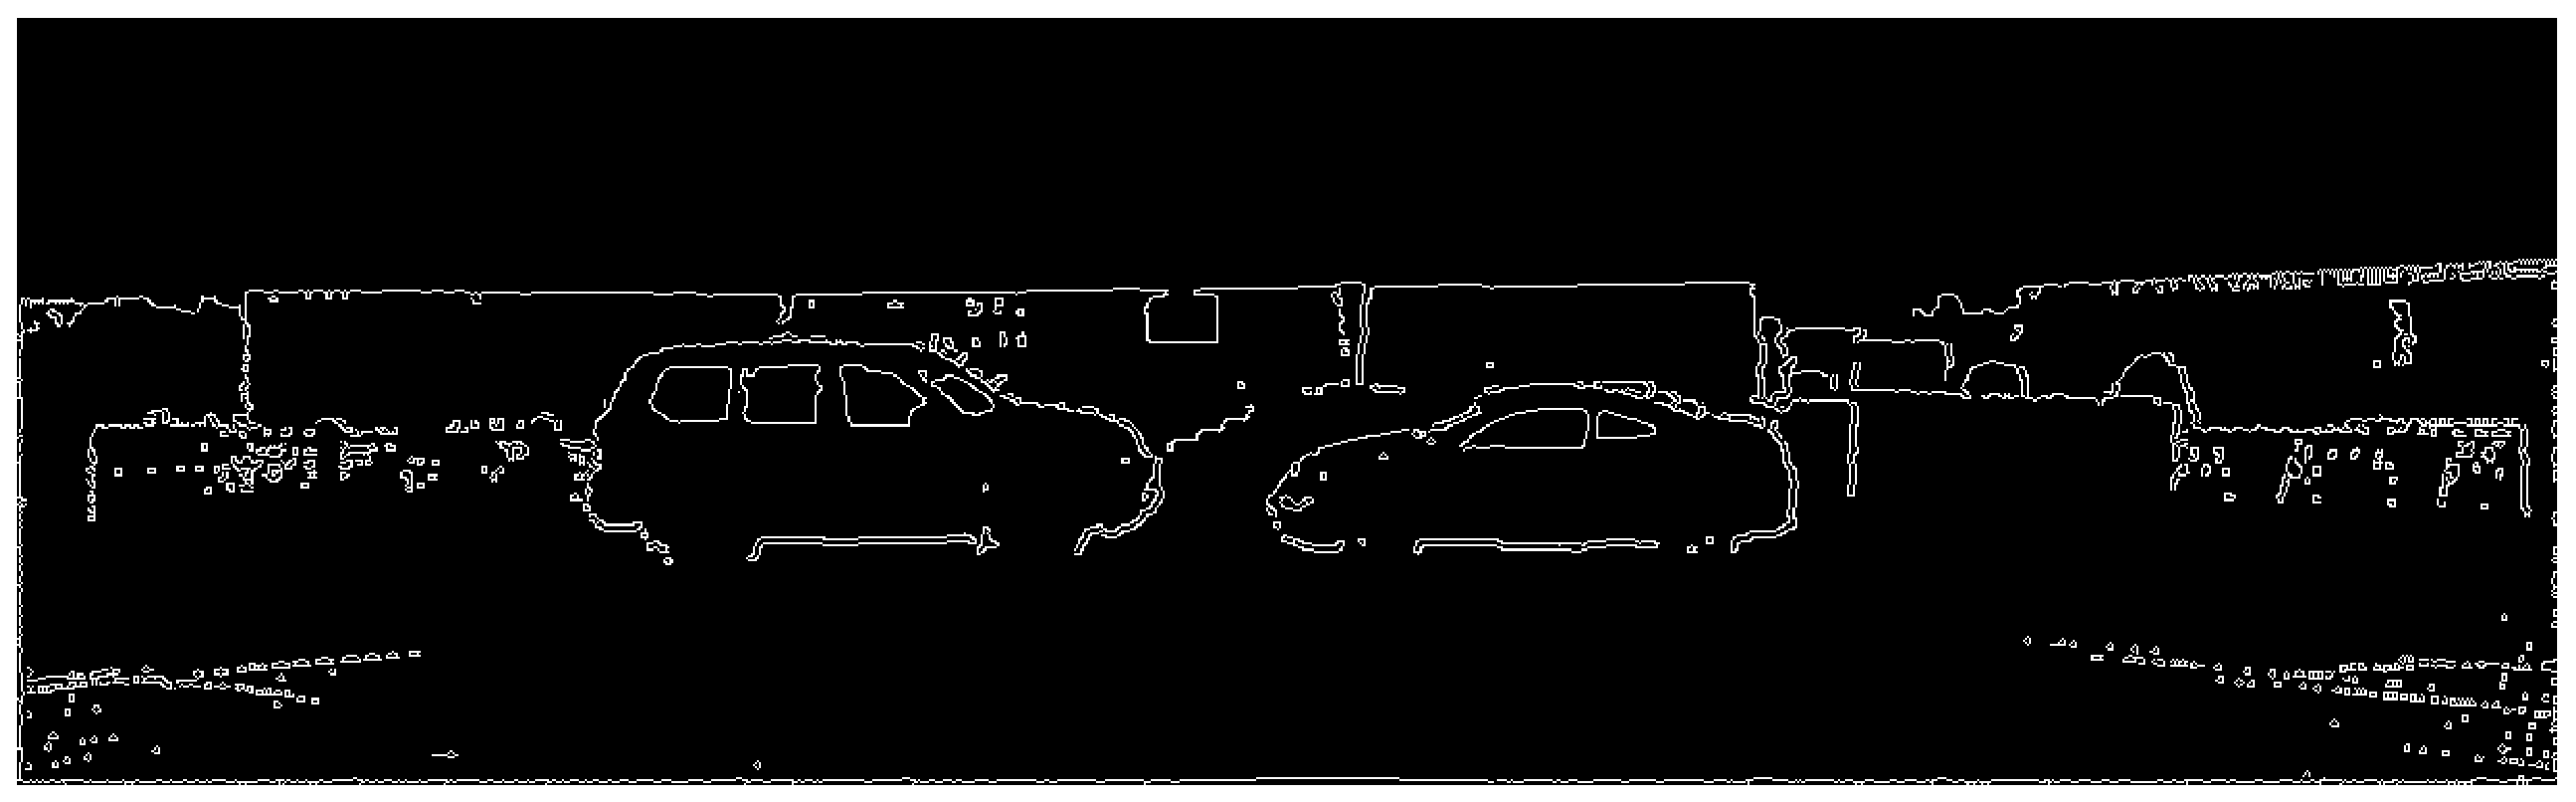
\includegraphics[scale=0.35]{mask5nodil}
\caption{Canny edge detection in an image}
\label{fig:edgenodil}
\end{figure} 

\subsection{Morphological Operations}
In addition to linear filters, there is another type of filters known as {\it non-linear filters}, whose output is a non-linear function of their input. 
In this type of filtering, unlike linear filters, the final value of a pixel is not necessarily 
a weighted combination of its neighboring pixels \cite{sze11}. 
{\it Median filter, Bilateral filter}, and {\it anisotropic diffusion} are all different types of non-linear filters. Non-linear filters are used for certain image manipulation 
and enhancement tasks, and are commonly used with a particular type of image called {\it binary
image} \cite{sze11}. Binary images, as their name indicates, consist of merely two pixel values, 0 or 1. These images are usually the outcome of filtering the values in an image 
by a certain threshold, thus changing each value to 0 or 1 based on the comparison against the threshold. Binary images are
widely used for {\it masking} operations in image processing \cite{sze11}. Due to extensive application of binary images, certain operations are usually employed to manipulate them. 
These operations are known as {\it morphological operations} \cite{ritt00}.
In morphological operations, the original image is convolved with a {\it structuring element}, also known as kernel. 
The structuring element is a mask (a binary image), normally smaller than the original image, 
with which different structures can be defined for later modification of the image. 
{\it Dilation} and {\it Erosion} are two of the most basic and widely used morphological operations in binary image processing.
These two operation are normally used for expansion and erosion of the shapes in the original image. 
In dilation, the structure element which is usually in form of a circle or square with the origin located at its centre, is superimposed on top of the original binary image.
By moving the structure element over the background pixels, each pixel belonging to the background, that 
is overlain by the centre of the structuring element, is replaced by foreground value if at least one of the pixels of the structuring element coincide with any pixel marked as foreground.
Erosion, which can be considered as the complementary operation of dilation, follows a similar process, with only the difference that structuring element is moved over foreground pixels and any
foreground pixels will be replaced by the background value if at least one pixel of the structuring element overlaps with a pixel marked as background.
Hence, we can state that dilation of the foreground is equivalent to erosion of the background \cite{ritt00}.
The dilation and erosion operations are illustrated in figures \ref{fig:dilate} and \ref{fig:erode}, respectively.

\begin{figure}[H]
\centering
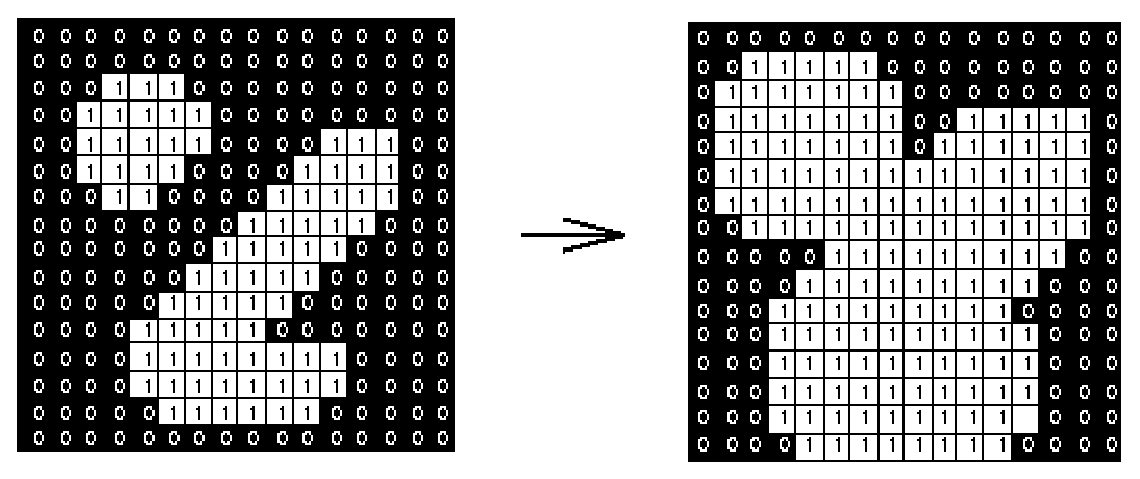
\includegraphics[scale=0.8]{diltbin}
\caption{Dilation operation}
\label{fig:dilate}
\end{figure} 

\begin{figure}[H]
\centering
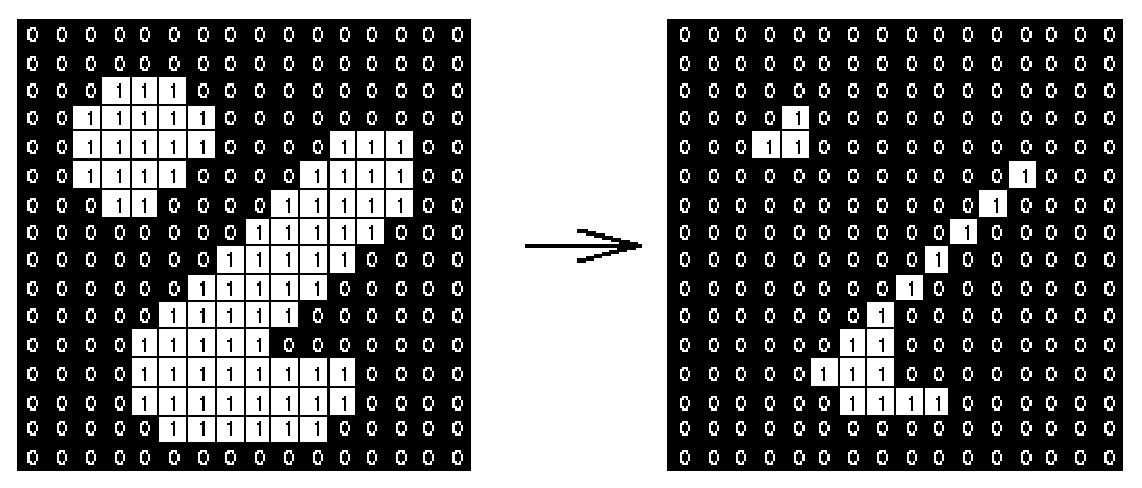
\includegraphics[scale=0.8]{erodbin}
\caption{Erosion operation}
\label{fig:erode}
\end{figure} 

The sample image shown in figure \ref{fig:edgenodil} is presented below after applying dilation on the detected edges in the image to expand the 
detected regions.

\begin{figure}[H]
\centering

\includegraphics[scale=0.35]{mask5dil}
\caption{Dilation of the detected edges in an image}
\label{fig:edgedil}
\end{figure} 






\chapter{Binocular Vision and Stereopsis}
\label{chap:BinocularVision}

\textit{Binocular vision} is a term used for the visual system of animals with two eyes \cite{how95}, and therefore, applies to the human visual system as well. 
Possessing binocular vision not only leads to a better perception of depth
of the surrounding environment, but also helps to better perform many visual tasks such as reading, object detection, interaction with surrounding objects such as grabbing and other manipulative 
tasks. The most significant advantage of possessing binocular vision is its influence on how the 3D environment; that is, the 
depth of surrounding objects relative to each other, 
is perceived by the visual system. This visual perception of depth in binocular vision is referred to as {\it Stereoscopic Vision}.
In the visual system, depth perception is a phenomenon that normally occurs though different types of cues and information existing in the surrounding environment. 
These pieces of information, known as {\it depth cues} in stereo vision, can be either monocular or binocular depth cues \cite{how95}.
To name a few instances of monocular depth cues, we can refer to motion parallax, lighting and shading, and apparent size. 
However, as previously mentioned, binocular cues which can only be perceived
by stereo vision, play a major role in the perception of depth. One of the most important binocular cues is {\it binocular disparity}, or {\it binocular parallax}. 
It should be noted that the effect of binocular parallax and motion parallax on depth perception are very similar to each other. 
In motion parallax, which is a monocular depth cue, the scene is viewed at different times by the observer moving from one side to the other, 
whereas in binocular parallax, the scene is viewed from slightly different viewpoints at
the same time by the visual system, while the observer is standing at a fixed position \cite{how95}.

\begin{figure}[!h]
\centering
\subcaptionbox{Motion Parallax}
[.4\linewidth]{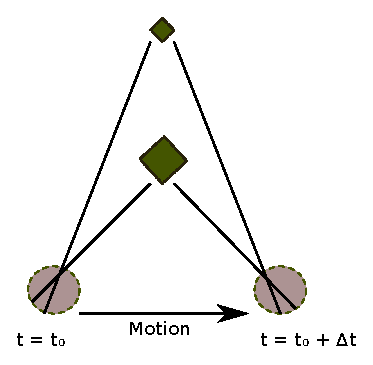
\includegraphics{Mparallax}}%
\subcaptionbox{Binocular Parallax}
[.4\linewidth]{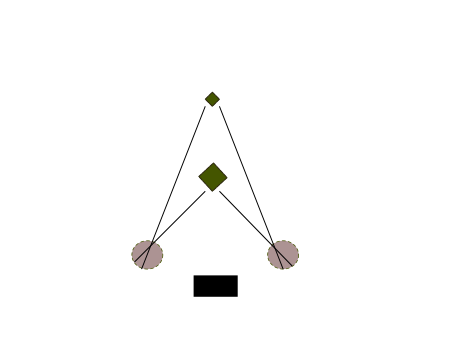
\includegraphics{Bparallax}}%
\caption{Motion parallax and binocular parallax difference}
\label{fig:parallax}
\end{figure}

%\begin{figure}[!h]
%\centering
%\begin{subfigure}[b]{7cm}            
%\frame{\includesvg[width=\textwidth]{Bparallax}}
%\caption{Interpolation for Data 1}
%\label{Fig:bp}
%\end{subfigure}
%
%\hspace{1cm}
%
%\begin{subfigure}[b]{7cm}
%\centering
%\frame{\includesvg[width=\textwidth]{Mparallax}}
%\caption{Interpolation for Data 2}
%\label{fig:mparallax}
%\end{subfigure}
%\caption{blah blah}\label{fig:bpmp}
%\end{figure}

Binocular disparity, which in fact arises from the spatial difference 
between the images of the same scene in the visual system, provides a relative perception of depth 
from the surrounding environment. This perception is known as {\it binocular stereopsis} \cite{how95}. 
Another important binocular depth cue is the eyes {\it vergence}, which is the simultaneous movement of the pupils in opposite directions in order to obtain a single vision of an object in the visual system. 
When focusing on an object, the optical axes of the eyes intersect on the object of interest resulting in an angle called vergence angle. Unlike many animals, the human visual system 
is capable of adjusting this angle based on the distance from the object.
In stereo vision, the locus of the points that yield a unified view of an object in the visual system is 
known as the {\it horopter}, and any point located on the horopter is usually called a 
{\it fixation point} \cite{binr83,how95}.
An important property of an object on the horopter is that no spatial difference
exists between the images of the fixated object between the two eyes; that is, the binocular disparity is zero \cite{how95}. 
Exploiting this property, the disparity of any other object in the scene can be estimated relative to the fixated object by inspecting two important factors: 
whether the object of interest is closer or further than the fixated object and then how much closer or further it is relative to the fixated object.
As a result, the binocular disparity provides a relative perception of depth of the surrounding environment.
In the geometry of stereopsis, the relative disparity between two objects is usually presented as 
angular disparity in degrees, radians, minutes of arc (arcminute), 
or seconds of arc (arcsecond). The relation between these measurements is as follows:

\begin{align}
1 arcmin &= \frac{1}{60} degree = \frac{\pi}{10800} radians \label{eq:arcmin} \\
1 arcsecond &= \frac{1}{60} arcmin = \frac{1}{3600} degree = \frac{\pi}{648000} radians \label{eq:arcsec}
\end{align}

\section{Stereopsis Geometry and Angular Disparity}

In the following section, we will describe how the angular disparity can be calculated utilizing the geometry of stereopsis \cite{binr83}.

\begin{figure}[!h]
\centering
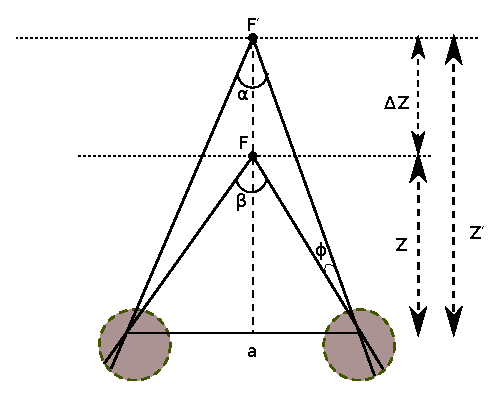
\includegraphics[width=0.5\textwidth]{binocular}
\caption{Binocular disparity}
\label{fig:stereopsis}
\end{figure} 

According to Figure \ref{fig:stereopsis}, we have:
\begin{align}
\theta &= \beta - \alpha\\
\alpha &= \frac{a}{Z^{'}}\\
\beta &= \frac{a}{Z}\\
Z^{'} &= Z + \Delta Z\\
\Rightarrow \theta &= \frac{a}{Z} - \frac{a}{Z^{'}}= \frac{a}{Z} - \frac{a}{Z+\Delta Z} \\
\Rightarrow \theta &= \frac{aZ+a\Delta Z-aZ}{Z(Z+\Delta Z)} = \frac{a \Delta Z}{Z(Z+ \Delta Z)}
\end{align}

When $\Delta Z$ is a small value compared to $Z$, the term $\Delta Z$ in denominator can be neglected without 
significant loss of accuracy. This results in
the approximate formula as follows:

\begin{align}
\label{eq:stac}
\theta = \frac{a \Delta Z}{Z^{2}}
\end{align}

Here, $a$ is the distance between the center of the pupils of the two eyes, which is known as interpupillary distance.
It should be noted that $a$, $Z$ and $ \Delta Z$ must all have the same units in this formula. 
This equation estimates the angular disparity in radian; in order to convert $\theta$ to arcseconds, 
according to the conversion rules presented in equation \ref{eq:arcsec}, it should be multiplied by:

\begin{align}
\frac {648000} {\pi} = 206,265
\end{align}

Studies show that the visual system capability to distinguish two objects at different depths relative to each other is limited to certain thresholds \cite{binr83,how95}.
This threshold, which is defined as the minimum detectable depth between two 
objects at difference distances, is known as {\it stereoacuity} which varies in different visual systems \cite{binr83,how95}. According to standard
stereo tests \cite{binr83}, the finest detectable disparity in the human visual system is approximately 10-15 arcseconds.
However, a more recent study on 60 subjects \cite{garn06} at different age groups, from 17 to 83 using standard stereotests, 
shows that the average stereoacuity for different age groups is as follows:

\begin{minipage}{\linewidth}
\begin{center}
\captionof{table}{Average stereoacuity for subjects of age 17 to 83}
\label{tab:stAcAge}
\begin{tabular}{ |c|c| }
\hline
\textbf{Age Range} & \textbf{Stereo Acuity (arcsecs)} \\ \hline
17-29 & 32 \\  \hline
30-49 & 33.75 \\ \hline
50-69 & 38.75 \\ \hline
70-83 & 112.5 \\ \hline
\end{tabular}
\end{center}
\end{minipage} \newline \newline

As can be seen, the stereoacuity for the the human visual system increases with the growth of the person's age; that is, 
the amount of error in the depth results 
is less perceptible in the visual system of the elders than the younger ones.
Using the values in equation \ref{eq:stac} along with the average interpupillary distance in the human visual system 
that is reported to be approximately $64$mm \cite{how95}, 
we can estimate the threshold for minimum detectable depth
between two objects based on their distance from the observer. \newline 

We have employed the concepts introduced in this chapter in the design of our evaluation model for an augmented reality system 
in outdoor environments.
In the next chapter, we will describe the design of our system and its components in more detail.

\chapter{Design of Evaluation Scheme}
\label{chap:System}

This chapter walks through the steps taken in order to build our evaluation system and describes its keys components in detail.

%Maybe should be moved to introduction?
\section{Design Criteria}

Since outdoor AR applications are the focus of this study, we have designed our evaluation model within this framework. Moreover, all the evaluation
metrics are measured based on the relevant factors described earlier in the previous chapters as perceived
by the human visual system.

%%%
%In these models, a pixel is considered as an \textit{outlier} if the error between the ground truth disparity and the disparity found by the solution is more than 
%a specified pixel threshold in the system, such as 2 or 3 pixels.
%They also provide separate masks for depth discontinuities and occluded regions, in addition to evaluating the whole image.
%%%

%However, both models take a general approach towards evaluating stereo algorithms; that is they have not been designed with an eye to the particular target 
%application.


%In other words, they mainly focus on the fundamental aspects of designing a stereo algorithm as a solution per se to \textit{efficiently}
%find the \textit{best matches} of corresponding pixels in stereo pairs. 
%This perspective may raise some questions for a punctilious researcher, such as:

%\begin{enumerate}
%\item What actually is an \textit{efficient} solution and on what basis is this \textit{efficiency} defined?
%\item What is a \textit{best match} of corresponding pixels and how can it be defined?
%\end{enumerate}


%In fact, these questions have compelled us to study the evaluation of the stereo matching solutions from a different point of view.
%In this design, we take steps towards an evaluation design which is based on the potential applications of stereo methods.
%This enables us to better define and adjust the criteria for \textit{efficiency} and 
%\textit{the best correspondence matches} while doing the evaluation.
%Since AR has attracted more attention in the past few years, 
%the evaluation scheme proposed in this study is designed based on outdoor AR applications which take advantage of
%stereo vision techniques to obtain a depth map of the surrounding environment. This map will then be used to
%integrate virtual objects in the scene that respect the occlusion property and the depth of the real objects in the scene. 
%In other words, the motivation of this research is to study the possibility and usability of integrating stereo vision techniques in an AR system, while considering the most
%important constraints that AR systems normally encounter \cite{liv05}.
%Move to Introduction Chapter

\section{New Evaluation Scheme}

In an augmented reality system, there are certain factors that would affect the functionality and effectiveness of the system \cite{liv05,kru10}, and therefore, 
should be carefully considered when designing and evaluating the system.
These factors, which correspond to the different components in an AR system, are related to the surrounding 
environment, technology and hardware constraints, or human factors in AR.
Figure \ref{fig:AR} illustrates a high level architecture of an AR system with its key components.

\begin{figure}[H]
\centering
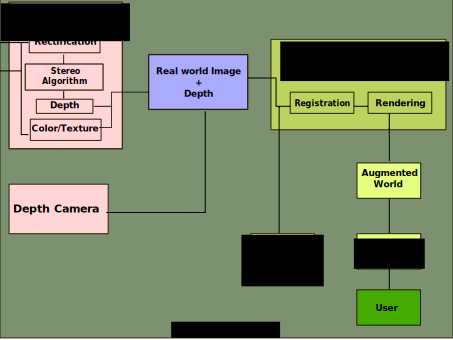
\includegraphics[scale=0.8]{AR}
\caption{High-level architecture of an AR system}
\label{fig:AR}
\end{figure} 

%Concentrating on the requirements of providing a real-time interaction between an AR system and the users, along with
%certain human factors that would affect the functionality of the system,
%has revealed the necessity of involving them in the evaluation of the stereo correspondence methods. Therefore, in order to 
%determine whether a stereo correspondence algorithm can meet the requirements of an AR application, we need an evaluation scheme which can properly assess 
%the \textit{efficiency} of the algorithm and the accuracy of its disparity results based on specific human factors in binocular vision and augmented reality.
%These factors are in fact the concepts related to real-time responsiveness of an AR system mentioned in \ref{chap:Introduction}, and binocular vision, stereopsis, human perception of depth, 
%and stereoacuity as thoroughly described in \ref{chap:BinocularVision}.

%In other words, we have proposed and desgined an evaluation scheme that studies some of the most important aspects of a system that consists of both
%AR and stereo vision components, thus enabling the designers to better evaluate the stereo correspondence solutions that will be intergrated 
%in the system.

In our design, unlike the Middlebury or Kitti benchmarks, we label a pixel in the disparity results as an \textit{outlier} if the angular
measurement, that is the stereoacuity, corresponding to the depth error between the ground truth and the estimated depth value by the 
algorithm is more than the minimum perceptible stereoacuities
for the human visual system as determined
by standard stereo tests \cite{binr83,garn06}. 
Moreover, we use the average stereoacuity for different age groups \cite{garn06} in our design to evaluate the performance of the algorithm for users 
at different ages; this makes the evaluation results more reliable and applicable to practical applications of AR.
In order to evaluate the efficiency of an algorithm and investigate whether it meets the requirements for being part of a real-time AR application, 
we have integrated a module in the evaluation process that reports on the average execution time of the algorithm for the input data.
The average number of outliers based on the specified stereoacuity thresholds and the average disparity error are also estimated during the evaluation process.

In addition, our model employs a particular approach which can be of specific value to practical AR applications. In this approach, we suggest that
it is prudent to focus the evaluation process on the particular regions of the disparity map rather than the whole image. The main hypothesis
is that salient edges caused by depth discontinuities, which also represent object boundaries and occlusion, are important depth cues for the human
visual system to better perceive the location of different objects in the 3D environment.
Therefore, more accurate depth results in these regions permits a higher quality combination of the depth map of the real world with the 
virtual depth of the synthetic objects that are part of the AR scene.
%In other words, in our model we have i
%exclusively applying and studying the evaluation process on those regions in the disparity map rather than the whole image.

\section{Design Overview}

Our evaluation model consists of the following key components:

\begin{itemize}
\item Stereo pairs, calibration data, and ground truth disparity (occluded or non-occluded) as inputs
\item Edge region masks generated from the ground truth disparity maps
\item Masked ground truth disparity
\item Full and masked disparity maps generated by the stereo algorithm 
\item Main evaluation module
\item Evaluation metrics output as data files and plots
\end{itemize}

It should be noted that some of these components, such as the masked ground truth, or the masked disparity maps 
can optionally be built during the process depending on the specific parameters set at the run time of each step.

Figure \ref{fig:higharch} shows the high level block diagram of our design.

\begin{figure}[H]
\centering
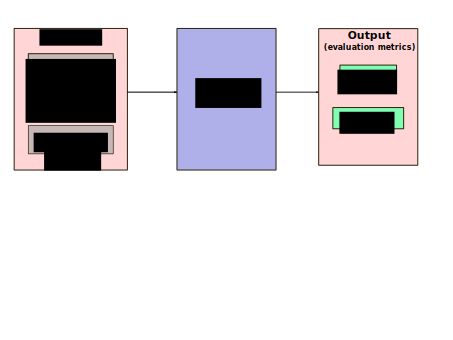
\includegraphics{EvalSyshigh}
\caption{High-level block diagram of the evaluation system}
\label{fig:higharch}
\end{figure} 
\noindent
A lower level architecture of our evaluation system is shown in Figure \ref{fig:lowarch}. This figure illustrates the 
sequence of the operations during the whole process. 

As can be seen in Figure \ref{fig:lowarch}, first the input data consisting of the stereo images, the ground truth disparity, and 
the calibration data are passed to the system.
Afterwards, the specified masks are created using a \textit{Canny} edge detector and a \textit{Dilation} operation with the appropriate parameters 
selected separately for each image.
After the corresponding disparity maps have been generated by the stereo algorithm and stored on the disk, 
they are passed to the evaluation module with the specified arguments.
Finally, the evaluation metrics are estimated and output through data files and plots to facilitate the evaluation of the stereo algorithm in the application
of interest; outdoor AR system.

\begin{figure}[H]
\centering
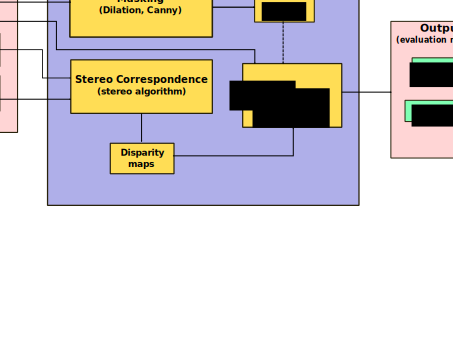
\includegraphics{EvalSyslow}
\caption{Low-level architecture of the evaluation system}
\label{fig:lowarch}
\end{figure} 

\section{Evaluation}
In this section, we break down the main evaluation component to its underlying modules. We will then look at the functionality of each
module in more detail.

As previously mentioned in this chapter, the results of the evaluation are presented through specific metrics which are as follows:

\begin{itemize}
\item{The average execution time}
\item{The average disparity error}
\item{The average number of outliers}
\item{The average stereoacuity}
\end{itemize}

The analysis of these metrics in the framework of an outdoor AR application will then allow for a practical evaluation of the stereo algorithm performance.
We will now explain how each of these metrics is measured in each module that builds up together the evaluation component in the system.

\subsection{The average Execution Time}
For each image pair, the time spent on generating the disparity results is estimated using the C++ function, \textit{clock()}. 
This function returns the number of clock ticks elapsed
since a program starts running. A division by the system-specific value \textit{CLOCK\_PER\_SECOND}, the number of clock ticks in a second, 
converts the value returned by \textit{clock} function into the time consumed by the CPU in seconds.
Getting the difference between the \textit{clock} values before and after a function call results in the execution time
of the particular function. 
We have applied this method in our implementation to estimate the execution time of the algorithm for each image pair. In the end, the mean of all
the values corresponding to different image pairs is taken to obtain the average execution time of the algorithm for the input dataset.

\subsection{The Average Disparity Error}
Two average disparity errors are calculated in our evaluation. One corresponds to the valid pixels in the ground truth, depending on what value is considered valid
in the ground truth disparity, and the other to
the valid pixels in the generated disparity which depends on the implementation of the stereo algorithm.
The valid ground truth disparity for the Kitti disparity maps, is a value greater than 0 and in the selected solutions, SGBM and ADCensus, 
values equal to or greater than 0 are considered valid.
To this end, for each validity criteria, the mean error between the ground truth disparity and the one found by the algorithm
is estimated for all the pixels in the image or merely the masked pixels depending on the availability of a mask.  

\subsection{The Average Number of Outliers}
Similar to the average disparity error, based on the validity criteria for disparity, 
two values are reported for this metric as a result of the evaluation. For this measurement, the relative depth error is first calculated by finding the corresponding depth values
for the ground truth disparity and the disparity generated by the algorithm in Equation \ref{eq:dispeq}. This value is then compared to the relative 
detectable depth threshold for the human visual system that is estimated using
equation \ref{eq:stac}. If the relative depth error is equal to or more than the detectable threshold in the human visual system,
the corresponding pixel is labelled as an outlier. Since we are using four different thresholds of stereoacuity corresponding to different
age groups in our evaluation, the estimated error is compared against each of these thresholds, and therefore,
four different values are eventually calculated. This process is repeated for all the pixels in the image or 
merely the pixels in the masked regions depending on the availability of a mask.
Considering the two validity criteria of pixels, eight values are reported at the end of the evaluation for the average number of outliers.

\subsection{The Average Stereoacuity}
The estimation of the average stereoacuity can be broken down into 3 steps:

\begin{enumerate}
\item Stereoacuity estimation based on the generated disparity for each image pair and the ground truth
\item Averaging the stereoacuity results over certain depth ranges in each image
\item Averaging the results from the previous step over all the images
\end{enumerate}
Corresponding plots are generated after the third step based on the final results.

According to the specific age ranges, different values are reported for the average stereoacuity
at the end of the evaluation. 
In order to estimate this metric, the depth values corresponding to both ground truth and the generated disparity by the algorithm are first
calculated using Equation \ref{eq:dispeq}. Subsequently, the difference between these values is used in Equation \ref{eq:stac} to calculate
the corresponding stereoacuity. This process is done for all the pixels in the image; or if a mask has been provided, 
it will be only applied to the pixels in the masked areas. Finally the results are output and stored in a separate data file for each image.
After conducting the first step on all the disparity maps corresponding to input image pairs, the second step starts by building a histogram of
the stereoacuity values over specific depth ranges. Using the output file containing the stereoacuity values 
from the first step for each disparity image, the corresponding histogram is constructed by defining the number of bins and their width.
In our design, the width of each bin determines the aforementioned depth range and is kept constant for all the bins.
Moreover, the number of bins along with their corresponding width determine the total distance over which the results
are estimated and subsequently examined.
\begin{equation}
\centering
Total\_distance = Number\_of\_bins * Width
\end{equation}
For outdoor applications of AR, these parameters are normally set to certain values so that the total distance can cover the medium to far 
depth fields; extending from 1.5 meters to more than 30 meters \cite{swa07}.
The results of the previous step, which are all stored in a single data file, are then passed to the last step. 
At this point, a histogram is built over the data from all the disparity images, which results in the average stereocuity
values within each specified depth range over all the images. 
It should be noted that the number of bins and their corresponding width at this point, are
similar to the histogram constructed in the the previous step.

\section{Platform}
The evaluation system was implemented on a Linux platform with Intel Core(TM) i7 3.20GHz CPU. 
We have used C++ as the high level language for implementing 
the core functions within the system, such as the main evaluation function, 
the masking process, and the other fundamental operations that are the building blocks of the system.
Furthermore, the Tool Command Language (TCL) has been used for all the scripts that wrap around the C++ functions,
to facilitate and accelerate the execution of each step in the process.

We described the main components of our proposed model in this chapter. Next, we will discuss the functionality of our system through different experiments.

\chapter{Evaluation}
\label{chap:Evaluation}
\renewcommand{\arraystretch}{0.5}

In this chapter, we will go through our experimental hypotheses, testing scenarios, experiments conducted on two sample 
stereo matching algorithms, SGBM and ADCensus, and the results with our
proposed evaluation system to assess the benefits of using our evaluation model for outdoor AR applications over the general-purpose evaluation models; 
the Middlebury and Kitti Stereo Evaluation.

\section{Stereo Dataset}
It should be noted that the stereo images we have used to conduct the experiments on stereo algorithms in our system,
are selected from the Kitti Stereo Dataset.
In contrary to the Middlebury dataset, the Kitti Stereo Project provides stereo images and ground truth disparity maps
that are taken from outdoor scenes under real circumstances. This property of sample images makes them more appropriate 
for evaluating the performance of the algorithms in outdoor AR applications, thus better meeting the objectives of this study.
We have selected 52 image pairs from the Kitti Stereo dataset based on different photometric and visual properties that are important
in stereo vision and an AR application. Some 
of these properties are listed as follows:
\begin{itemize}
\item Light and shading, that is the scenes including bright, dim, and dark regions
\item Various depth ranges, that is including near field, medium field and far field objects  
\item Depth discontinuity and occlusion
\item Well textured and not properly textured regions
\end{itemize}


\section{Methodology}

Before going through the explanation of the experiments to assess our evaluation model, we restate our main research question in this
study to better justify our hypotheses and the experiments defined for their validation. 
As mentioned earlier in chapter \ref{chap:Introduction}, our main objective is to investigate whether using 
stereo matching techniques to generate the depth map of the 
surrounding environment in an outdoor AR application can meet the requirements of the AR system. 
Therefore, our experiments focus 
on assessing those aspects of our evaluation model that assist to better answer this question.
As a result, our first attempt towards evaluating our model is to investigate and demonstrate whether the results of the evaluation process 
are properly measured and presented in the framework of the important factors in an outdoor AR application.
After confirming this property, which is the key property of our model, we investigate the effect of our proposed masking 
approach on the evaluation results. Moreover, we present how the methods are evaluated in the framework of 
real-time interactive AR systems.
We also explain how the evaluation and comparison of the methods is done in our model with some
experiments on the sample stereo matching algorithms.

\section{Hypotheses}

We have defined a set of hypotheses to evaluate our proposed design. These hypotheses are as follows:

\begin{itemize}
\item \textbf{Hypothesis 1}: \emph{Our model evaluates and demonstrates 
the performance of the stereo matching algorithm in the framework of 
the outdoor augmented reality applications.} 
Unlike the Middlebury and Kitti benchmarks which are considered general-purpose evaluation models, 
our system can particularly evaluate the algorithms in the framework of an 
outdoor augmented reality application to facilitate the process of determining
the proper method for using in the AR system for a high quality real-time generation of the depth map of the surrounding environment from 
the user's point of view.

\item \textbf{Hypothesis 2:} \emph{Observing, evaluating, and consequently 
refining the areas near the depth edges in an image are more important in an AR application.}
Salient edges caused by depth discontinuities, 
which can also represent the object boundaries and occlusion, are one of the 
most important depth cues that helps the observer to better perceive the depth of different objects in the scene. In other words, the areas near the edges corresponding to depth discontinuities
in a scene are more important to the human visual system for perception of depth in an AR application and, therefore, the disparity 
errors in these regions can be detected easier by the HVS. Therefore, we argue that in our model, which has the property of masking and evaluating the results for
these particular regions,
the evaluation results can be of great value to an outdoor AR application.

\item \textbf{Hypothesis 3:} \emph{Our system is better than other evaluation models for assessing the performance of the algorithm in
real-time AR applications.}
Other evaluation models, the Kitti and Middlebury benchmarks, do not evaluate and report on the efficiency of the algorithms
with respect to their execution time. On the other hand, our system is capable of examining and evaluating an algorithm 
based on its execution time and, therefore, can report on its efficiency for real-time AR applications.

\item \textbf{Hypothesis 4:} \emph{The trade-off between the accuracy and the running time of the stereo algorithms can be effectively evaluated 
in the framework of an outdoor AR application through our system.} 
Nearly all the solutions to the problem of stereo correspondence have been dealing with the trade-off between the accuracy of the results and the running time.
Therefore, most of the solutions focus only on improving one of these aspects in the final results. Some methods use certain post processing techniques to refine the 
disparity results in the end, thus improving the accuracy, whereas the others propose particular approaches that can be implemented on the GPU.
Due to the importance of both metrics in an outdoor AR application, we argue that the trade-off between these metrics can be effectively analyzed in our evaluation system.


\end{itemize}

The experiments designed to validate these hypotheses are explained in the following sections.

\section{Experimental Environment and Settings}
Experiments were carried out on a Linux machine with Intel Core(TM) i7 3.20GHz CPU. 
Although ADCensus is proposed as a GPU-based solution to the problem of stereo correspondence, 
we have used the CPU implementation of both algorithms in all the experiments.
The set of parameters used at different steps of the evaluation are presented in the following sections.
It should be noted that these parameters were kept constant for all the images and experiments. However, if a parameter is changed during an experiment for specific
reasons, it will be explicitly mentioned in the description of the experiment.

\subsection{Masking}
In order to build the masks in our system, the OpenCV Canny edge detector and Dilation are used.
Canny have been used to detect the depth edges in the ground truth disparity map, and the dilation operation 
for expanding the detected edge regions in the masking process. The extent to which the regions are expanded
is determined by the number of iterations in the dilation operation. Table \ref{tab:candilparam} shows the parameters used in the Dilation
and the Canny edge detection. However, the \textit{minimum threshold} in Canny is tuned and selected separately for each image 
since the threshold should change depending on the scene.

{\footnotesize
\begin{minipage}{\linewidth}
\begin{center}
\captionof{table}{Masking Parameters}
\label{tab:candilparam}
\begin{tabular}{ |c|c| }
\hline
Dilation\_iterations & 10 \\  \hline
Canny\_apertureSize & 3 \\ \hline
\end{tabular}
\end{center}
\end{minipage} \newline
}

The ground truth disparity maps in the Kitti stereo dataset are generated by a 3D laser scanner, thereby resembling
a point cloud map of discrete disparity values. This property of the disparity images 
can be problematic for the masking process since it can result in many small streaks as the edges.
Therefore, before applying any edge
detection on the image, we need to first fill the gaps by interpolating the values and obtain a smoothed ground truth disparity.
This can be achieved by applying a dilation operation.
In our implementation, we have used the OpenCV dilation operation with different number of iterations for each image, that is set depending on the scene 
and the original ground truth disparity, to obtain a fully dense disparity map. 
The new disparity images are then stored on the disk for further use.
However, it should be noted that the dilated disparity images are only used in the construction of the masks when detecting the depth
edges in the image.
%However, it should be noted that the ground truth disparities used for the related comparisons and calculations 
%in the evaluation process, are the original disparity images before being dilation.

\subsection{Stereo Algorithms Settings}
The parameters for each algorithm used in our experiments to generate the disparity
maps are kept constant over all the images in the dataset. These parameters are presented in Tables \ref{tab:sgbmparams} and \ref{tab:adcparams} 
for SGBM and ADCensus, respectively.

{\footnotesize
\begin{minipage}{\linewidth}
\begin{center}
\captionof{table}{SGBM Parameters}
\label{tab:sgbmparams}
\begin{tabular}{ |c|c|c|c|}
\hline
SADWindowSize & 9 & disp12MaxDiff & 2 \\ \hline
uniquenessRatio & 10 & P2 & 3*9 \\ \hline
speckleWindowSize & 100 & speckleRange & 2 \\ \hline
\end{tabular}
\end{center}
\end{minipage} \newline
}

Other parameters not mentioned in the table are considered with their default values.

{\footnotesize
\begin{minipage}{\linewidth}
\begin{center}
\captionof{table}{ADCensus Parameters}
\label{tab:adcparams}
\begin{tabular}{|c|c|c|c|c|c|c|c|}
\hline
$\lambda_{AD}$ & 10 & $\lambda_{Census}$ & 30 & $L_{1}$ & 34 & $L_{2}$ & 17 \\ \hline
$\tau_{1}$ & 20 & $\tau_{2}$ & 6 & $\pi_{1}$ & 1.0 & $\pi_{2}$ & 3.0 \\ \hline 
$\tau_{SO}$ & 15 & $\tau_{S}$ & 20 & $\tau_{H}$ & 0.4 & & \\  \hline
\end{tabular}
\end{center}
\end{minipage} \newline
}

The minimum and maximum disparity values are also kept constant for each image pair in both algorithms; however, the maximum 
disparity differ for each image pair as the scenes are different
and objects are located at different depth fields.
The minimum disparity is set to $0$ for both algorithms. The maximum disparity for each image pair is selected based on the maximum value in their
corresponding ground truth disparity. The only restriction to consider here is to choose a value greater than or equal to 
the maximum disparity of the ground truth that is a multiplication of 16. This constraint
is implied by the implementation of SGBM algorithm.

\subsection{Evaluation Params}
In our evaluation model, due to the large amount of data which grows as more images are added to the input selection, 
plots are generated by taking the average of the results over all the images. As mentioned in the previous chapter, this average results from two steps; 
first, getting the average of the stereoacuity over specific
depth ranges for each image and then getting the average of the values from the previous step over all of the images. This operation finally results in a single plot
that demonstrates the average stereoacuity within specific distance.
The averaging operations at this step are implemented by building histogram over the resulting data. 
In our experiments, we set the number of bins to $100$ and the width of each bin to $0.5$. Therefore, the first averaging is conducted over distances of $0.5m$ 
in each image and the maximum distance over which the results are 
examined is $50m$.

%\section{Assumption}
%\textbf{Talk about camera quality and display resolution}

\section{Experiments}
In this section, we discuss the experiments conducted to evaluate the system and investigate the validity of our hypotheses.

\subsection{Evaluation in Augmented Reality Framework}

In this experiment, the disparity maps 
were generated for fifty-two image pairs with both SGBM and ADCensus algorithms. 
After generating the corresponding disparity maps for all the images, 
the evaluation process was conducted on each map separately.

Sample plots corresponding to one of the stereo pairs, shown in Figure \ref{fig:img5},
over the masked areas are displayed in Figures \ref{fig:imgmsk5} and \ref{fig:imgfull5}, respectively.

\begin{figure}[h!]
\centering
\subcaptionbox{Left image}
[.5\linewidth]{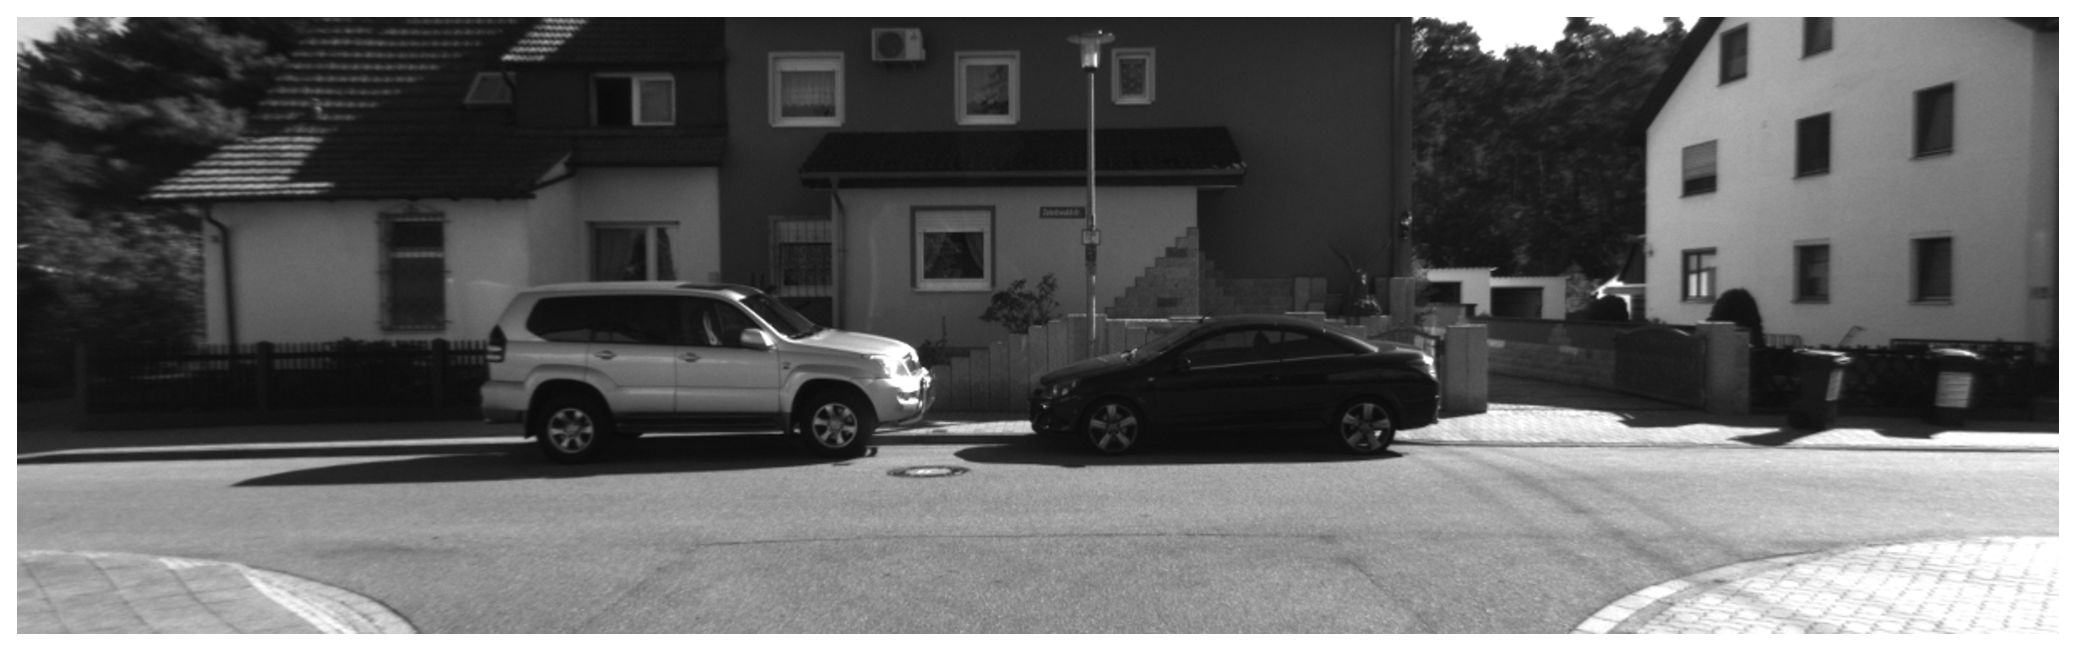
\includegraphics[scale=0.21]{000005L}}%
\subcaptionbox{Right image}
[.5\linewidth]{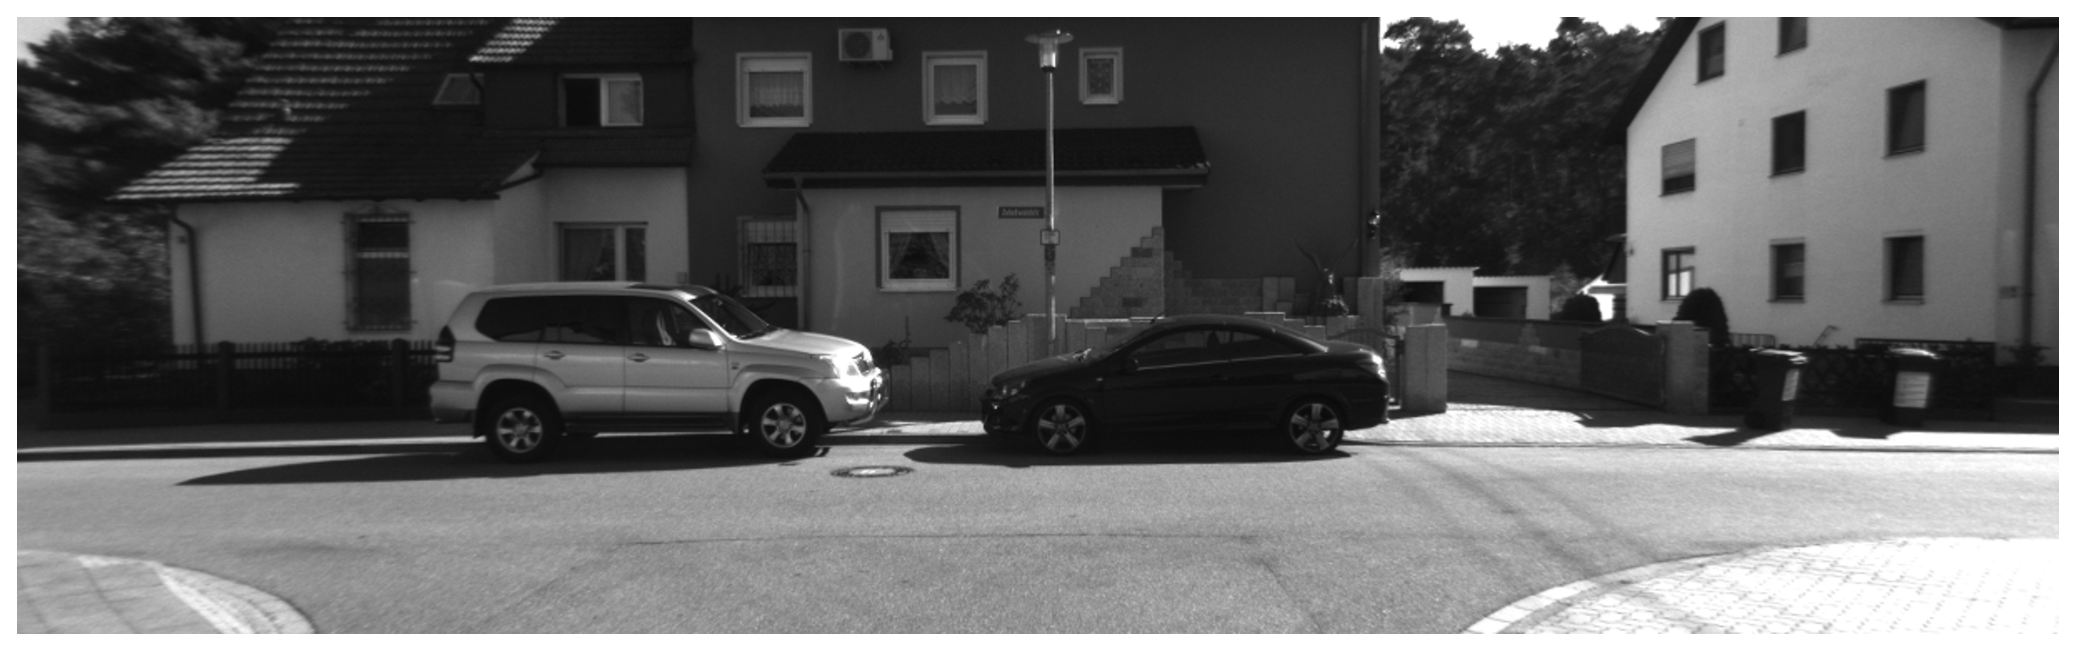
\includegraphics[scale=0.21]{000005R}}%
\caption{Sample stereo image from the Kitti dataset}
\label{fig:img5}
\end{figure}

\begin{figure}[H]
\centering
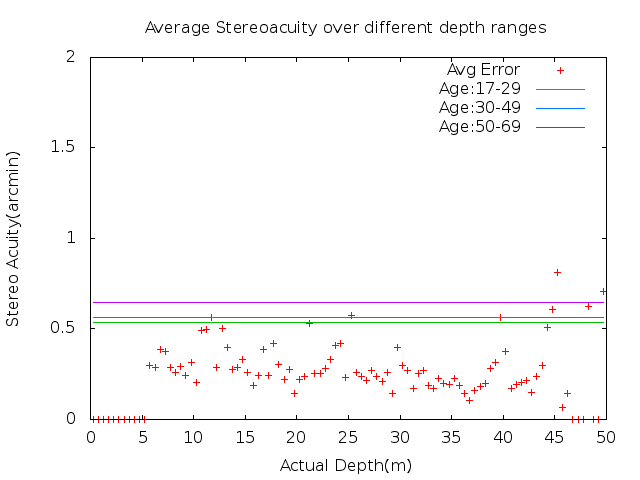
\includegraphics[scale=0.8]{sgbmimg5pix3msk}
\caption{Average disparity error over distance by SGBM}
\label{fig:imgmsk5}
\end{figure} 

\begin{figure}[H]
\centering
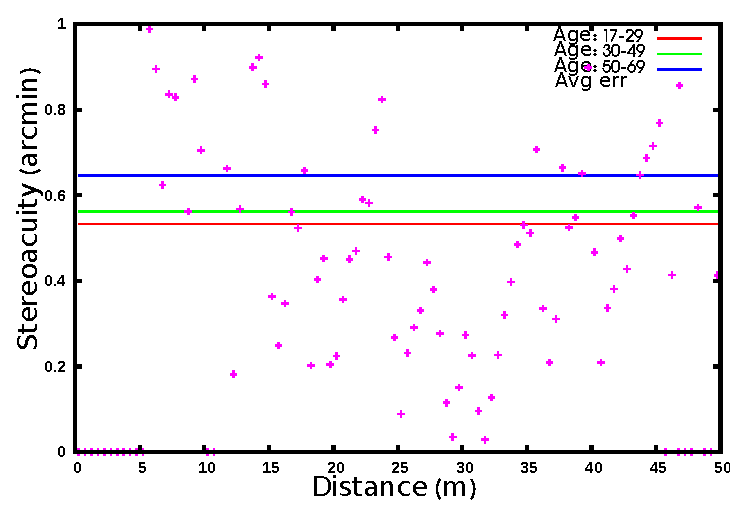
\includegraphics[scale=0.8]{adcimg5pix3msk}
\caption{Average disparity error over distance by ADCensus}
\label{fig:imgfull5}
\end{figure}

\noindent
The corresponding mask, Figure \ref{fig:msk}; masked ground truth, Figure \ref{fig:gtmsk}; and
the masked disparity images generated by SGBM and ADCensus, Figures \ref{fig:5mdispsgb} and \ref{fig:5mdispadc} 
are shown below.

\begin{figure}[H]
\centering

\includegraphics[scale=0.35]{5msk}
\caption{The mask of depth edges and their surrounding regions}
\label{fig:msk}
\end{figure} 

\begin{figure}[H]
\centering

\includegraphics[scale=0.35]{5gt}
\caption{Masked ground truth}
\label{fig:gtmsk}
\end{figure} 

\begin{figure}[H]
\centering

\includegraphics[scale=0.35]{5mdispsgb}
\caption{Masked disparity by SGBM}
\label{fig:5mdispsgb}
\end{figure} 

\begin{figure}[H]
\centering

\includegraphics[scale=0.35]{5mdispadc}
\caption{Masked disparity by ADCensus}
\label{fig:5mdispadc}
\end{figure} 

\noindent
Figures \ref{fig:mskmapsgbm} and \ref{fig:mskmapadc} show the average results over all the disparity images for both SGBM and ADCensus, respectively.

\begin{figure}[H]
\centering
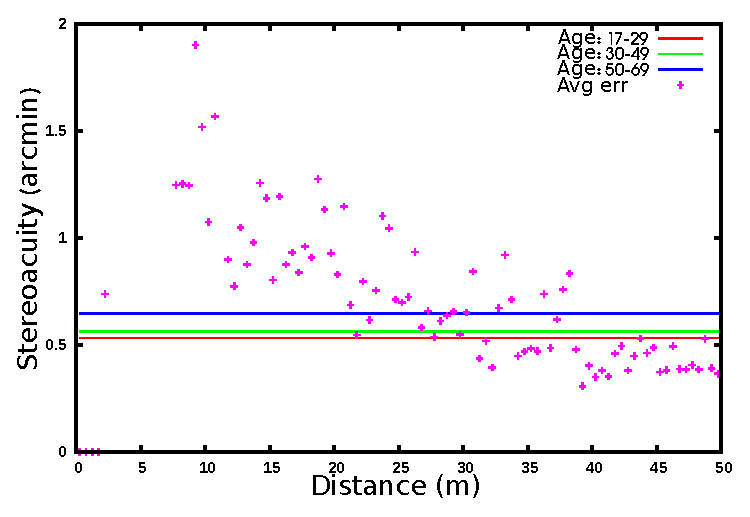
\includegraphics[scale=0.8]{sgbmmsk1000}
\caption{Average disparity error over all the images by SGBM}
\label{fig:mskmapsgbm}
\end{figure} 

\begin{figure}[H]
\centering
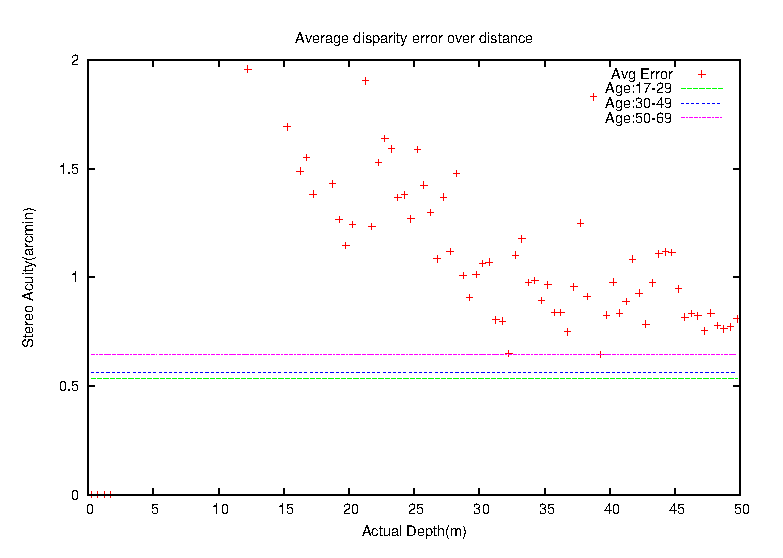
\includegraphics[scale=0.8]{adcenmsk1000}
\caption{Average disparity error over all the images by ADCensus}
\label{fig:mskmapadc}
\end{figure} 

As can be seen, the average results displayed in the previous plots contain sparse points and 
do not demonstrate any consistent pattern. When we investigated the cause of this large variation, we found that in
the results of both algorithms, there are some disparity values which differ from the ground truth 
by a considerable amount and yet have not been invalidated by the
algorithm. We assume that these types of outliers can be easily removed from the set by applying a post processing filter, or 
they will be eventually culled out by the 3D renderer in the AR system. 
%Therefore, we have added another filtering condition to our evaluation module is similar to the approach employed by the
%Kiiti and Middlebury stereo evaluation. 
In order to filter out the disparity values which largely differ from the ground truth disparity, we have integrated another 
step in our evaluation process. This step is similar to the strategy used in the Kitti and Middlebury evaluation models.
In this step, the estimated disparity error is initially compared to a more generally defined threshold, for instance a threshold of 3 pixels.
This comparison allows for only those values of disparity with an error less than or equal to the specified threshold to 
move on to the next steps of the evaluation. It should be noted in our design, the specified threshold is defined as a run-time variable. 

The additional filtering had a significant impact on the evaluation results. In fact, a consistent pattern was observed in the final plots after filtering out the
outliers with large differences. The results are displayed in
figures \ref{fig:mskmapsgbm} and \ref{fig:mskmapadc}.

\begin{figure}[H]
\centering
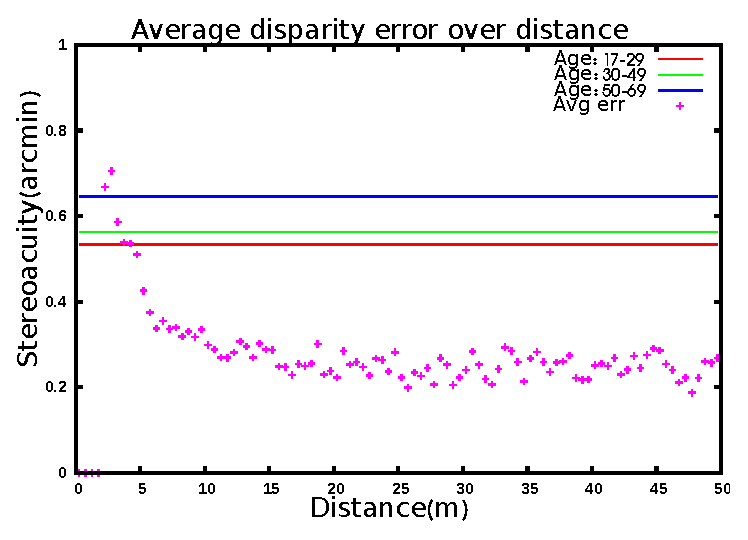
\includegraphics[scale=0.8]{sgbmmsk3}
\caption{Average disparity error over all the images by SGBM}
\label{fig:mskmapsgbm}
\end{figure} 

\begin{figure}[H]
\centering
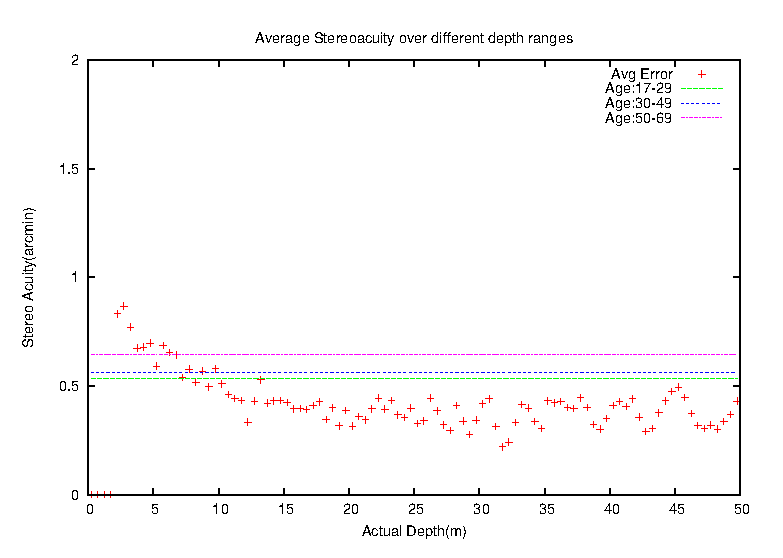
\includegraphics[scale=0.8]{adcenmsk3}
\caption{Average disparity error over all the images by ADCensus}
\label{fig:mskmapadc}
\end{figure} 

In these plots, a cross point below a stereoacuity threshold (straight lines) implies that the average error in the disparity values estimated 
by the stereo matching 
algorithm is imperceptible to the human visual system. However, a value higher than the threshold indicates that
the error cannot be ignored and should be resolved to achieve a better alignment between the virtual and the 
real world in the AR application of interest. Moreover, as can be seen most of the errors
fall below the standard stereoacuity value corresponding to older ages; indicating that they are not perceptible to the visual system of the people at these 
particular ages.

The zero values in the plots imply that either there is no object within the corresponding range or the disparity value estimated by the algorithm
is equal to the ground truth disparity; however, since the average of the results has been taken over all the images, it is more likely that 
the zero values indicate no object within the particular range.

As can be seen in the results, SGBM performs better in finding more accurate corresponding matches 
compared to ADCensus, as most of the error points fall below the standard stereoacuity lines. Moreover, the plots show that in both methods 
the significant amount of error
corresponds to the near field objects, within the first 5 meters. This range of the depth field can be considerably important in some applications,
such as the ones involving certain manipulative tasks.

\subsection{Depth edges and Occlusion}
In order to examine the effect of evaluating certain regions of the disparity image instead of the whole image, 
we estimated the average error both for the masked areas and the whole disparity map. 
Results of SGBM are shown in Figures \ref{fig:sgbmfull3} and \ref{fig:sgbmmsk3}.

\begin{figure}[H]
\centering
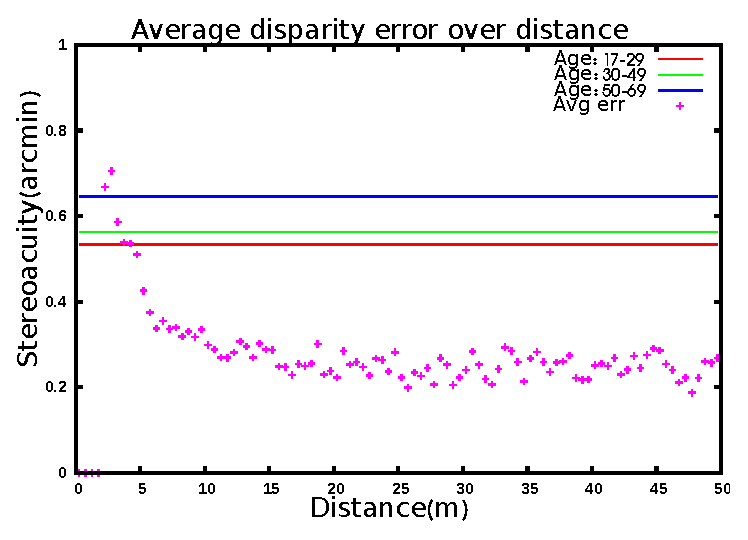
\includegraphics[scale=0.8]{sgbmmsk3}
\caption{Average disparity error over masked areas by SGBM}
\label{fig:sgbmmsk3}
\end{figure} 

\begin{figure}[H]
\centering
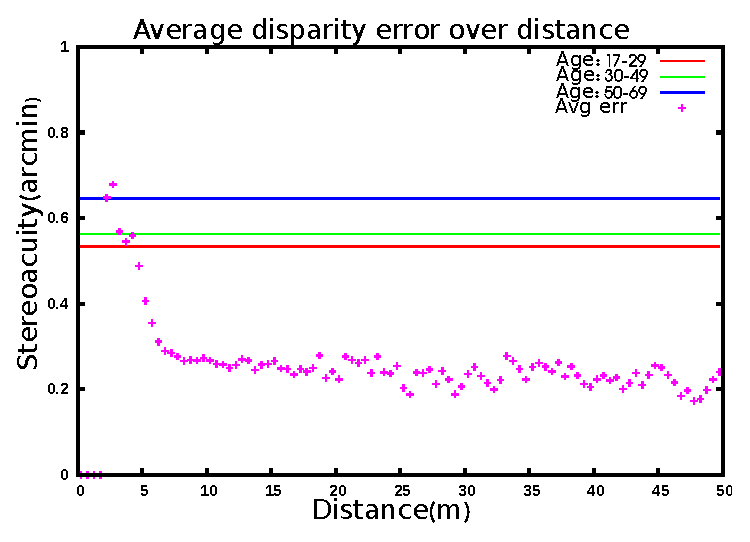
\includegraphics[scale=0.8]{sgbmfull3}
\caption{Average disparity error over the whole image by SGBM}
\label{fig:sgbmfull3}
\end{figure} 

The plots show that the average error over the masked regions, that is near the depth edges, is very similar to the results over the whole image. 
This may imply that there is no additional benefit in the inspection of these regions. 
However, this might be merely an indication of the performance of the selected algorithms and can be better analyzed by evaluating more algorithms 
within our model.
In either case, we argue that, due to the importance of occlusion and areas near depth discontinuities to the HVS in AR applications, 
it is reasonable to focus more on the depth edges and their surroundings when designing or employing a stereo matching technique for an AR application.

\subsection{Average Outliers}
In this experiment the average outliers were measured for both algorithms. 
The values for both validity criteria mentioned in chapter \ref{chap:System}, valid pixels in the ground truth and generated disparity, 
are presented in Tables \ref{tab:outlmsk} and \ref{tab:outlfull} for each age group. For simplicity, we have labelled the valid pixels
in the ground truth and the generated disparity with \textbf{vG} and \textbf{vD}, respectively.
Figure \ref{fig:outlbar} also represents a chart of all the results for one of these validity criteria, when the grount truth disparity is valid.

%{\footnotesize
\begin{minipage}{0.8\linewidth}
\begin{center}
\captionof{table}{Average outliers for the masked regions}
\label{tab:outlmsk}
\begin{tabular}{ |c|c|c|c| }
\hline
Algorithm & Age & Avg\_Outliers(vG) & Avg\_Outliers(vD) \\ \hline
\multirow{4}{*}{SGBM} & 17-29 & 0.12 & 0.16 \\
& 30-49 & 0.11 & 0.15 \\
& 50-69 & 0.09 & 0.12 \\
& 70-83 & 0.0012 & 0.0016 \\ \hline
\multirow{4}{*}{ADCensus} & 17-29 & 0.23 & 0.32 \\
& 30-49 & 0.22 & 0.31 \\
& 50-69 & 0.18 & 0.27 \\
& 70-83 & 0.002 & 0.003 \\ \hline
\end{tabular}
\end{center}
\end{minipage} \newline \newline
%}

\begin{minipage}{0.8\linewidth}
\begin{center}
\captionof{table}{Average outliers for the whole image}
\label{tab:outlfull}
\begin{tabular}{ |c|c|c|c| }
\hline
Algorithm & Age & Avg\_Outliers(vG) & Avg\_Outliers(vD)  \\ \hline
\multirow{4}{*}{SGBM} & 17-29 & 0.11 & 0.14 \\
& 30-49 & 0.10 & 0.12 \\
& 50-69 & 0.08 & 0.09 \\
& 70-83 & 0.005 & 0.007 \\ \hline
\multirow{4}{*}{ADCensus} & 17-29 & 0.27 & 0.39 \\
& 30-49 & 0.26 & 0.37 \\
& 50-69 & 0.22 & 0.32 \\
& 70-83 & 0.002 & 0.003 \\ \hline
\end{tabular}
\end{center}
\end{minipage} \newline

Results show that in both cases, the masked regions and the whole image, SGBM has less number of outliers than ADCensus, indicating that
SGBM generates a more accurate disparity map as perceived by the human visual system.
Another observation is that in SGBM, the number of outliers over the masked regions are more than the outliers over the whole image, whereas in ADCensus the
opposite behavior is observed. This implies that SGBM, as a solution per se, generate less accurate results
near the depth discontinuities and occluded regions compared to the other areas in the image.
On the other hand, ADCensus per se, results in more accurate disparity values near the depth edges compared to the other regions in the image and 
tends to preserve the occluded regions. This only indicates that, despite the better performance of SGBM over ADCensus according to the
experimental results, in cases where only one of these solutions is available, it is reasonable to consider this behavior to employ the method
in the right application based on the requirement of the target system for the accuracy of the depth results in different regions; in other
words, it is important to first investigate which regions of the image are more important in the context of the target application.
%whether the accuracy near the depth discontinuities and preserving the occlusion is more important than the
%other regions in the image or not.
For instance, ADCensus performs better in an application where the areas
near the depth discontinuities and occlusion are more important than the rest of the image, such as image compositing for layering visual elements
on the scene, compared to application scenarios where obtaining an accurate, dense disparity map for all the regions in an image is essential.

\begin{figure}[H]
\centering
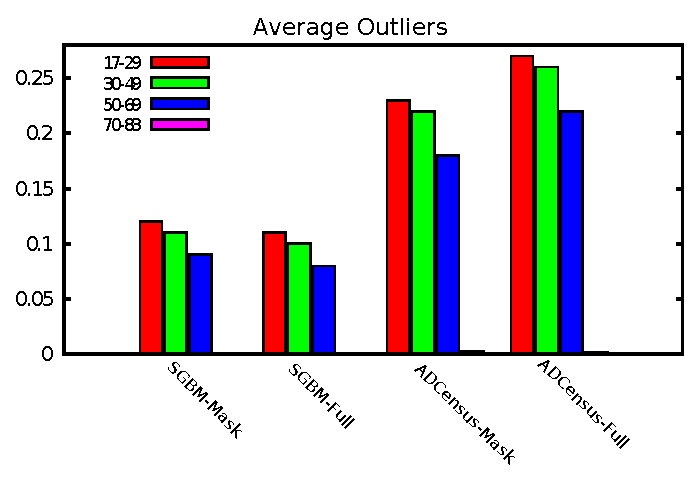
\includegraphics[scale=0.9]{outlchart}
\caption{Average disparity error for the masked regions - not refined}
\label{fig:outlbar}
\end{figure} 

%Furthermore, in SGBM the number of outliers over the masked regions are more than the outliers over the whole image, whereas in ADCensus the
%opposite behavior is observed; that is the number of outliers over the masked regions are less than 
%the whole image. This implies that ADCensus performs better in the areas of depth edges and their surroundings than other regions.
%Therefore, it is better to be employed in the applications where preserving the object boundaries and occluded areas
%is adequate and more important than the other regions in the image, such as image compositing for layering visual elements
%on the scene. However, this metric per se
%cannot be an indicator of the suitability of the solution for any target application and should be considered along with the other
%relevant metrics. 

We should note that the reason the number of outliers for the valid pixels in the generated disparity is more than the outliers for the valid pixels
in the ground truth is that in our implementation, the counter for the number of pixels in the ground truth image 
is incremented whenever a disparity pixel in the ground truth is labelled as valid, regardless of other conditions in the process; 
however, the counter for the number of pixels in the generated disparity
is only incremented whenever the disparity value is valid and the amount of disparity error is less than the specified pixel threshold in the evaluation process, thus resulting
in a smaller denominator of the fraction in the estimation of the average outliers for the criteria of valid pixels in the generated disparity map and, therefore, a larger 
average value in the end.

\subsection{Average Disparity Error}
The average disparity error have also been estimated in the evaluation process for both pixel validity criteria. However, the resulting values
were similar for both cases and, therefore, only one value is reported in the following table for this metric.

\begin{minipage}{0.8\linewidth}
\begin{center}
\captionof{table}{Average disparity error}
\label{tab:avgerr}
\begin{tabular}{ |c|c|c| }
\hline
Algorithm & Region & Avg\_DispErr \\ \hline
\multirow{2}{*}{SGBM} & Full & 6.58 \\ \cline{2-3}
& Masked & 7.81 \\ \hline
\multirow{2}{*}{ADCensus} & Full & 4.49 \\ \cline{2-3}
& Masked & 4.74 \\ \hline
\end{tabular}
\end{center}
\end{minipage} \newline

As can be seen, ADCensus results in less average disparity error than SGBM. This difference is likely caused by the various refinement steps
implemented in the ADCensus algorithm which do not exist in SGBM.
As a result, despite the larger number of outliers in ADCensus than SGBM as measured in the previous experiments,
ADCensus attempts to decrease the difference between the resulting disparity value and the ground truth disparity, thus generating a smoother disparity patches
within different regions of the image.

\subsection{Real-time Execution}
In another experiment, we estimated the average execution time for both algorithms. Results show that the average execution time over all the images 
for SGBM and ADCensus are $0.54$ and $272.82$ seconds, respectively.
Considering the requirements of having an interactive real-time AR system \cite{hertz00}, the processing time of each frame should not be more than 0.06-0.08 seconds.
Although the current implementation of SGBM could be used when the real world scene remains stable for approximately one second, it can be safely concluded that
none of these algorithms meet the requirements of a real-time interactive AR system.
This suggests that the GPU-based solutions are better techniques to achieve the processing speed required for the real-time 
interactive applications of AR.

\subsection{Effect of Refinement}
In this experiment, we studied the effect of the post processing steps, also referred to as the \textit{refinement steps}, 
in the stereo algorithms on the accuracy of the results in our evaluation criteria. 

Refinement is usually the last step in a stereo correspondence algorithm because it attempts to decrease the 
number of wrong matches or the error after the disparity results have been found, thus requiring the outliers to be first detected in the results. 
The detection of the outliers occurs through a check known as left-right consistency check in a stereo matching algorithm. In this check, the disparity map for both
the left and right image is first calculated. Then, if a pixel in the left image, based on its disparity value, corresponds to a pixel in the right image
that does not map back to it, it will be labeled as an outlier. This description can be formulated as follows:
\begin{align}
D_{L}(p) \neq D_{R}(p-(D_{L},0))
\end{align}
\noindent
Where $D_{L}(p)$ is the disparity function for the left image and $D_{R}$ is the disparity function for the right image.

For simplicity, we will refer
to this check as LR check in this report.
In our implementation of ADCensus, we have the LR check and its subsequent refinement steps triggered with a flag.
Therefore, when the flag is not set, neither the check nor the refining steps are triggered in the algorithm.
To investigate the effect of the refinement on the final results, we used 
ADcensus in this experiment with the LR flag set to zero, generating the disparity results for the image pairs, and evaluating the results.
The results for both cases, refined and not refined, over the masked regions and the whole image are shown below.

\begin{figure}[H]
\centering
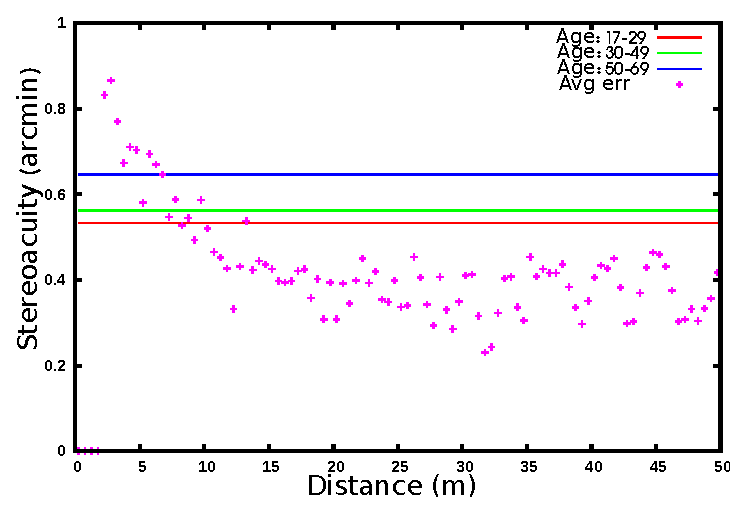
\includegraphics[scale=0.8]{adcenmsk3NoLR}
\caption{Average disparity error for the masked regions - not refined}
\label{fig:adcmnoLR}
\end{figure} 

\begin{figure}[H]
\centering
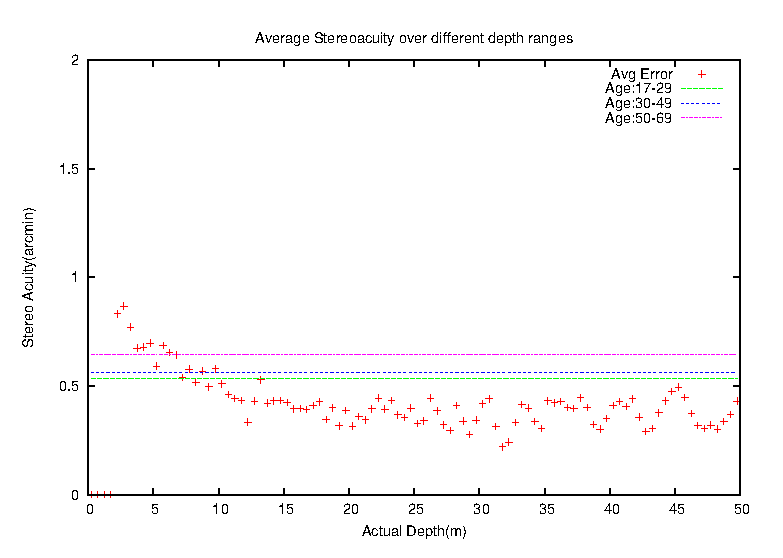
\includegraphics[scale=0.8]{adcenmsk3}
\caption{Average disparity error for the masked regions - refined}
\label{fig:adcm3}
\end{figure} 

\begin{figure}[H]
\centering
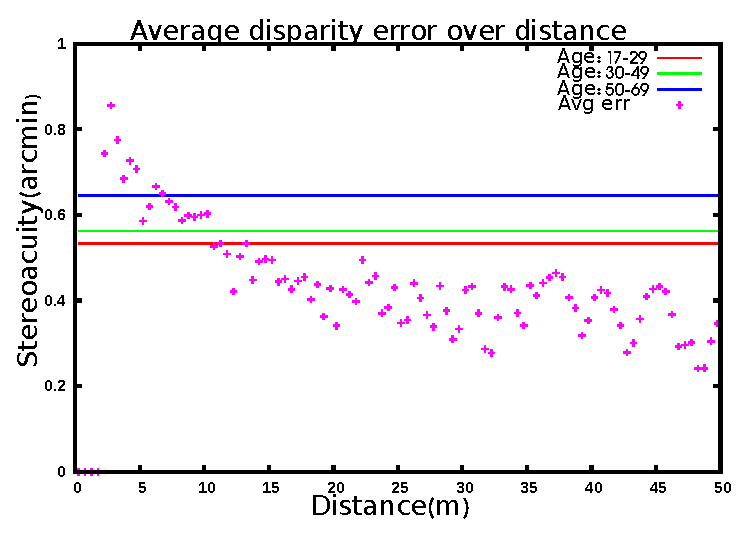
\includegraphics[scale=0.8]{adcenfull3NoLR}
\caption{Average disparity error for the whole image - not refined}
\label{fig:adcfnoLR}
\end{figure} 

\begin{figure}[H]
\centering
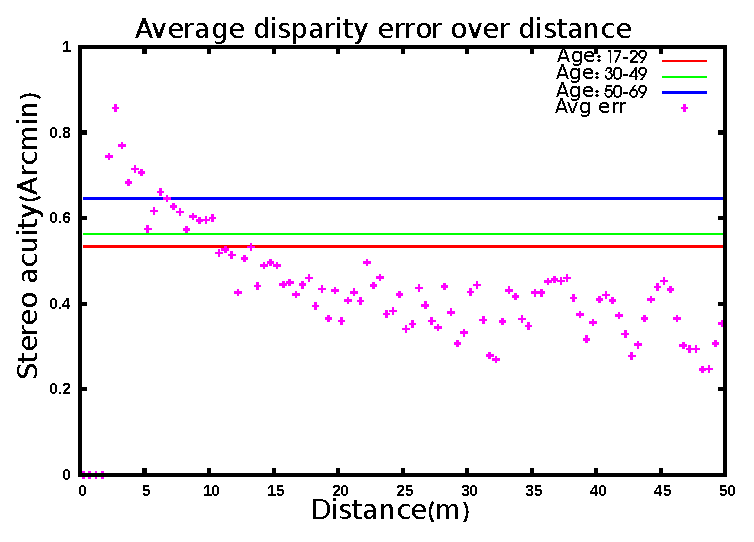
\includegraphics[scale=0.8]{adcenfull3}
\caption{Average disparity error for the whole image - refined}
\label{fig:adcf3}
\end{figure} 

As can be seen in the plots, the evaluation results in our specific criteria 
are not significantly different from the results of the algorithm when LR check and refinement were triggered
and only a few average values have slightly changed. We have marked a few of these values with a blue circle in Figures \ref{fig:adcmnoLR} and \ref{fig:adcfnoLR}.

We also estimated the average execution time, the average disparity error, and the average outliers in this experiment. The results for 
the average error and outliers are shown in the tables below.

\begin{minipage}{0.8\linewidth}
\begin{center}
\captionof{table}{ADCensus average disparity error - no refinement}
\label{tab:adcerrNref}
\begin{tabular}{|c|c|}
\hline
Region & Avg\_DispErr \\ \hline
Masked & 5.59 \\  \hline
Full & 5.29 \\ \hline
\end{tabular}
\end{center}
\end{minipage} \newline

\begin{minipage}{0.8\linewidth}
\begin{center}
\captionof{table}{ADCensus average outliers - no refinement}
\label{tab:adcoutlNref}
\begin{tabular}{ |c|c|c|c| }
\hline
Region & Age &  Avg\_Outliers(vG) & Avg\_Outliers(vD)  \\ \hline
\multirow{4}{*}{Masked} & 17-29 & 0.23 & 0.33 \\
& 30-49 & 0.22 & 0.31 \\
& 50-69 & 0.18 & 0.27 \\
& 70-83 & 0.002 & 0.003 \\ \hline
\multirow{4}{*}{Full} & 17-29 & 0.27 & 0.39 \\
& 30-49 & 0.26 & 0.37 \\
& 50-69 & 0.23 & 0.32 \\
& 70-83 & 0.001 & 0.002 \\ \hline
\end{tabular}
\end{center}
\end{minipage} \newline

Figure \ref{fig:outlnoref} shows a comparison between the results of ADCensus with and without the refinement 
for one of the validity criteria, when the ground truth disparity is valid. As can be seen, no significant decrease is obtained in the number of outliers.

\begin{figure}[H]
\centering
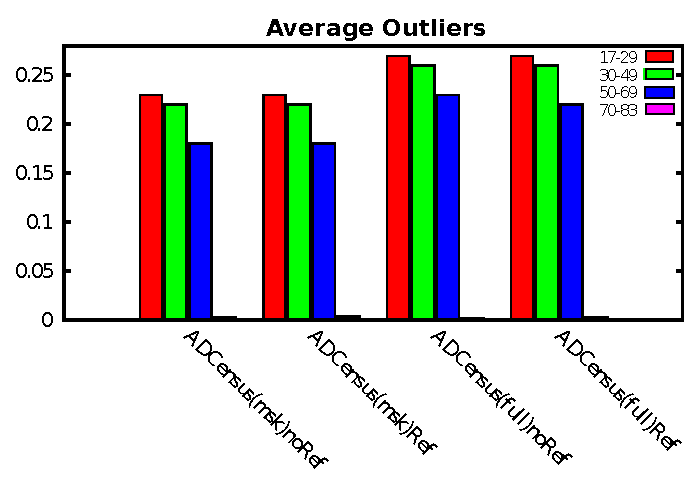
\includegraphics[scale=0.9]{adcrefNoref}
\caption{Average disparity error for the masked regions - not refined}
\label{fig:outlnoref}
\end{figure} 

The average execution time was approximately $147.84$ seconds which is nearly half the running time of the algorithm with the LR check and refinements triggered. 
Comparing these results to the ones presented in Tables \ref{tab:outlmsk}, \ref{tab:outlfull}, and \ref{tab:avgerr} a slight decrease in the amount of errors and 
almost no change in the number of outliers is observed.
Analyzing the results in this experiment, we can conclude that despite the considerable rise in the execution time of the algorithm, no significant
accuracy is achieved in our evaluation criteria through refinement of the disparity results; therefore, the execution of ADCensus without any LR check and
refinement step is more beneficial to an AR application in outdoor environments.

\section{Hypotheses Validation}
Next, we will review our hypotheses mentioned earlier in this chapter and discuss their validity in the light of our experiments and their results.

\begin{itemize}
\item \textbf{Hypothesis 1}: \emph{Our model evaluates and demonstrates the accuracy of a stereo matching algorithm in the framework of 
outdoor augmented reality applications.} 
As can be seen in the results of the experiments, our system employs a systematic approach for the measurement and demonstration of different 
evaluation metrics in the framework of an outdoor augmented reality application. 
In our system, the disparity error, which is the most important metric for the accuracy of the disparity results, 
is converted to a certain measurement, stereoacuity, that is relevant and applicable to the human visual
system and its perception of depth. We evaluated two stereo matching methods in our system and analyzed their performance in terms of
the accuracy of the depth map for an outdoor AR application. Due to the application-oriented design of the system, we could comment on the suitability of each method
for an AR application in outdoor environments. As a result, we can claim that our evaluation model is more appropriate for the evaluation of the solutions 
in an outdoor AR system than the conventional evaluation systems.

\item \textbf{Hypothesis 2:} \emph{Observing, evaluating, and consequently 
refining the areas near the depth edges in an image are more important in an AR application.}
The results of our experiments on two sample stereo matching solutions showed no significant difference between the evaluation metrics corresponding to the whole image and
the regions of the depth edges and their surroundings, thereby implying that there may be no specific benefit into the analysis of these particular regions 
in an outdoor AR application.
However, due to the importance of these regions as depth cues to the human visual system for the perception of the 3D location of the surrounding 
objects in an environment, we argue that more solutions should be tested within our evaluation model 
to be able to certainly approve or disapprove this hypothesis. 

\item \textbf{Hypothesis 3:} \emph{Our system performs better than the the conventional evaluation models for assessing the performance of a stereo algorithm in
Real-time AR applications.}
As explained in the design of our model and demonstrated in the experimental results, the execution time of the algorithms 
is estimated and evaluated in the system based on the requirements of having a real-time and interactive augmented reality application.
In the experiments, we evaluated the running time of the two sample stereo matching algorithms which proved to be inefficient in both cases for 
a real-time augmented reality application. Through this property, we can claim that the evaluation results through our system is more beneficial to AR applications
than the conventional evaluation models which do not take this important aspect of the solutions into account.

\item \textbf{Hypothesis 4:} \emph{The trade-off between the accuracy and the running time of the stereo algorithms can be effectively evaluated 
in the framework of an outdoor AR application through our system.} 
In one of the experiments, we focused on the trade-off between the accuracy of the results and the running time of the algorithm by studying the effect
of the post processing steps, also referred to as refinement steps, on the evaluation metrics. Results on ADCensus showed that integrating these steps in the algorithm
does not significantly improve the accuracy of the results in the framework of an outdoor AR system; on the other hand, it causes a considerable increase in the execution
time of the algorithm which is not beneficial to a real-time and interactive AR system. The results of this evaluation indicates that the trade-off between the accuracy 
of the results and the execution time of the algorithm, which normally exists in nearly all the stereo matching solutions, can be effectively analyzed 
through our evaluation system. The conventional evaluation models lack this property which is of great importance to certain applications, such as applications of AR.

\end{itemize}

\section{Detectability of Depth in AR}
According to different studies \cite{dras96, kru10,azuma01}, some other factors such as issues associated with the environment, display device, and capturing device
can also affect the perception of depth in the visual system. As a result, the ability to detect the difference in depth 
does not merely depend on how accurate the stereo correspondence algorithm can estimate the depth values and detect the steps in depth.
In order to investigate the validity of this statement, we conducted another experiment. In this experiment we defined some stereoacuity thresholds,
or better to phrase as the detectable depth difference
in terms of stereoacuity. In order to find the minimum threshold to start with, we attempted to find the 
minimum disparity change in the grount truth disparity images. To this end, we move through horizontal scanlines in each image and 
compute the difference between the values of consecutive pixels, which is, in fact, an indicator of the detectability of the difference in depth. 
After finding the minimum value in each image, a global minimum is sought between all the computed values from different images.
The value we found for image size of $1242\times375$ and the focal length of $721$ millimeters was $0.0022$ arcmins.
After finding this minimum and defining our thresholds, we apply a nearly similar operation on the disparity results from each of the sample algorithms.
In this process, while moving through each image, for those pixels whose generated disparity is close to the ground truth disparity, within a pre-defined pixel threshold, 
we estimate their depth difference from their following pixel
in the ground truth and compare the value to each of the specified thresholds; if this value is less than a threshold, then we check to see whether
the stereo algorithm has also detected different values for the corresponding pixels. 
In case of detection, we increment a counter corresponding to each threshold.
This process is repeated for different images and, finally, the average of the detected changes is estimated for each specified threshold.

\begin{alltt}
\textbf{ADP}; START
      define StAc\_thresh;
      for all pixels p in the image; do
         if (\( |disp\sb{gt}-disp\sb{gen}|<pix\_thresh\));
            \(pix\_count++\);
            \(diff = |disp\sb{gen\sb{i}}-disp\sb{gen\sb{i+1}}|\);
            \(depth\sb{gt\sb{i}} = \frac{focal\_length \times baseline}{disp\sb{gen\sb{i}}}\);
            \(depth\sb{gt\sb{i+1}} = \frac{focal\_length \times baseline}{disp\sb{gen\sb{i+1}}}\);
            \(depthDiff = |depth\sb{gt\sb{i}}-depth\sb{gt\sb{i+1}}|\);
            \(stAc\_detected = \frac{pupil\_distance*depthDiff}{depth\sb{gt\sb{i}}\sp{2}}\);
            for each threshold \textit{thr} in StAc\_thresh; do
               if (\(stAc\_detected<thr\))
                  if (\(diff>0\))
                     \(detected[thr]++\);
                  fi
               fi
            end for
      end for
      for each threshold \textit{thr} in StAc\_thresh; do
         \(Avg\_detected[thr] = detected[thr]/pix\_count\);
      end for
\textbf{ADP}; END
\end{alltt}
The results for both algorithms are shown in Figure \ref{fig:algthresh}.

\begin{figure}[H]
\centering
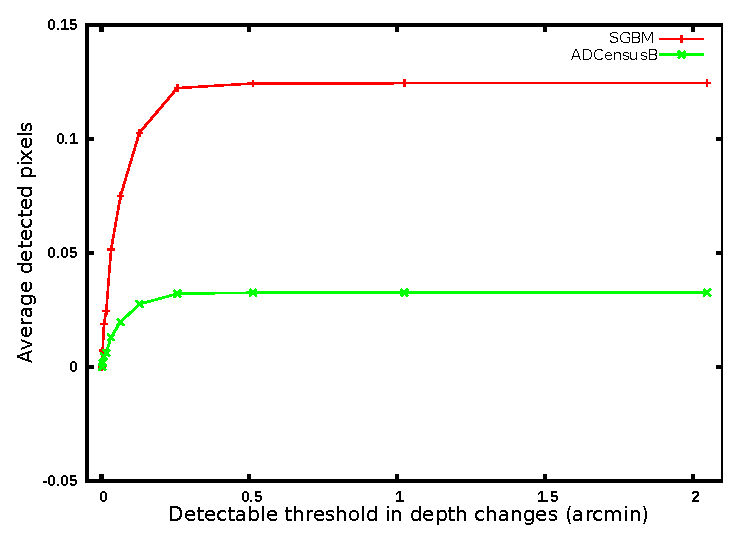
\includegraphics{algthreshBoth}
\caption{Average detected changes for different stereoacuity thresholds}
\label{fig:algthresh}
\end{figure} 

As can be seen in these plots, for both algorithms, the average detected changes in disparity differences starts to converge at the value of approximately $0.4$ arcmins.
We also observe that for the values below this threshold the average detected changes are much lower and for some values, such as the minimum detectable threshold in ground truth,
both algorithms are not capable of detecting any change. 
This implies that, regardless of the accuracy resolution of the algorithms, which is $1/8$th of a pixel for SGBM and $1/16$th of a pixel for ADCensus and approximately equal to
$0.6$ arcmins and $0.3$ arcmins, respectively, for Kitti images based on the camera parameters and the geometrical relation presented in Figure \ref{fig:camResolution} and 
Equation \ref{eq:algResolution}, some changes in 
depth in the real world are still not be detected by the algorithm. This effect might be related to the sensor resolution, that is, the resolution of the capturing device or the effect
of noise. Therefore, in order to achieve better detectability of depth changes by the algorithms, that is, to obtain a lower threshold
which is closer to the actual resolution of the implemented algorithm, using higher resolution devices is also essential.
However, our previous experimental results show that despite various types of error caused by the capturing device, noise, or the discretization limit of the stereo correspondence 
algorithm in the estimation of disparity values, in many cases depending on the distance of the object from the observer,  
the error in the results will not be perceptible to the HVS in an outdoor AR
application.

\begin{figure}[H]
\centering

\includegraphics{camRes}
\caption{Resolution of image in angular disparity}
\label{fig:camResolution}
\end{figure}
\noindent
Where, $w$ is the image width and $f$ is the focal length of the capturing device.
For the imge size of $1242\times375$ and focal length of $721$, and based on the resolution of SGBM and ADCensus in the estimation of the disparity values, 
the detectable disparity difference in terms of stereoacuity is as follows:

\begin{align}
\label{eq:algResolution}
SGBM: \theta &= \arctan (\frac{\frac{1}{8}}{721}) = 0.0099 degrees \times 60 \frac{arcmins}{dgrees} = 0.59 arcmins \\
ADCensus: \theta &= \arctan (\frac{\frac{1}{16}}{721}) = 0.0049 degrees \times 60 \frac{arcmins}{degrees}= 0.29 arcmins
\end{align}

\chapter{Conclusion}
\label{chap:Conclusion}
In this chapter, we succinctly mention our contributions in this study and specify some interesting paths for future 
research and improvement to our proposed system.

\section{Contributions}
Due to the emergence of various applications which combine different techniques in computer vision 
to build a practical system, developing testbeds which are particularly designed for the evaluation of different components in the criteria of the important factors
in the target application is essential.
Nowadays, building practical AR applications is a challenging problem due to the various constraints that these systems normally face. We believe that
addressing these constraints and attempting to find the efficient solutions are propitious research directions.

In this research, we suggest that stereo correspondence methods can be used in outdoor AR systems
as a practical alternative to conventional and inefficient technologies, 3D laser scanner or depth cameras, for obtaining the depth map 
of the surrounding environment, but only if a real-time implementation is used.
This approach, that is, employing stereo correspondence solutions, requires an evaluation scheme which can effectively evaluate the stereo correspondence methods 
while taking the target application into consideration. As a result, the available
evaluation models, Middlebury and Kitti, will not be sufficient for an effective evaluation of the solutions.
Therefore, our main contribution in this study, is proposing an application-oriented evaluation scheme that is designed in the light of the most important
factors in an outdoor AR system. Since humans are the ultimate users of an AR system, we have focused on the relevant factors in the human visual system
that are important for the real-time interaction with the augmented world and the perception of depth of the surrounding environment. We have integrated
specific metrics in our evaluation system which are measured and subsequently evaluated in the framework of an outdoor AR application, thus effectively
analyzing the performance of the solutions in terms of their accuracy and efficiency, that is its execution time, for the target application. These metrics are
the average stereoacuity over distance, the average number of outliers, the average disparity error and the the average execution time. We also suggest that some specific areas 
in a scene are of more importance to AR applications in outdoor environments. Due to the importance of depth discontinuities and occlusion as depth cues to the human visual system,
we define these regions as the depth edges and their surroundings in the scene. Although our experiments did not prove to be sufficient to investigate the validity of this hypothesis,
we would still hypothesize that these regions are worthy of being studied in AR applications.
In addition, the trade-off between the accuracy and the running time of a stereo algorithm can be studied through our system in the framework of an outdoor AR system, thus
better determining the net benefit of certain post processing steps to the target application.

In conclusion, the experimental results in most cases showed the effectiveness of our approach for evaluation of the stereo solutions in outdoor AR applications, which encourages
further research in this particular direction to improve this model in more useful aspects.
Next, we will mention some aspects in which we believe the system can be improved.

\section{Future Work}
This evaluation model can be improved in a few aspects that we will discuss here.
As seen in the experiments, we could not certainly determine the importance of the depth edges in the scene to the outdoor AR application and subsequently their consideration in the evaluation 
of the stereo algorithms. We believe that a solid conclusion can be made by evaluating more stereo matching solutions
within our model and observing the results in the masked regions and the whole image. A better approach to make a more solid hypothesis and design a better 
evaluation is through conducting a user study in which user is wearing see-through AR glasses and a synthetic object is placed in particular regions in the scene based on the depth map generated by the stereo correspondence algorithm. The amount of error and its affect on the human perception of depth must then be observed and evaluated in this study. 

Another interesting aspect of improvement is a rigorous study on the effect of other factors that can affect the effectiveness and 
usability of the outdoor AR system and, therefore, 
are important to be considered in the evaluation of the method that is used to obtain the depth map of the surrounding environment. 
To name some of these factors we can refer to
the resolution of the display devices in the AR system and the effect of contrast and brightness. 
For this evaluation, different video streams or stereo images can be captured using devices with different resolutions 
and from different scenes where the effect of shadow and lighting is well depicted. A segmentation algorithm can then be used to 
segment specific regions with different effects of shadow and lighting and the depth results by the algorithm in these areas can then be estimated and evaluated. 
A user study, similar to the one mentioned previously, can also be conducted here to observe and evaluate the effects of the depth results and 
their errors on the HVS in each case.  
A more complete list of the important factors in AR can be
found in the survey on the perceptual issues in augmented reality by Kruijff et al. \cite{kru10}.

There are different post processing techniques in computer vision that can be used to refine the disparity results, such as color segmentation and plane fitting, 
anisotropic diffusion, and common smoothing filters as Gaussian filter. However, most of these techniques can considerably increase the execution time of the algorithm.
A study of different refining methods and their effect on the accuracy and the running time of the algorithm in the framework of a particular application, 
such as an outdoor AR system, is an interesting topic to investigate and can be a valuable asset to many industrial applications.

Another interesting subject for studying is focusing on the evaluation of the existing GPU-based stereo matching techniques in our system.
Investigating their suitability for integration in an outdoor AR system based on their running time, which is expected to be considerably less 
than many CPU-based solutions, 
and the accuracy of their results in the light of the relevant factors to an outdoor AR system can be an interesting subject for research.

Furthermore, we believe that it will be of specific value to
assess the benefits of our proposed model and its applicability to other applications of augmented reality, such as underwater environments, in which the environmental 
noise is more significant and is more challenging to address. 

We certainly encourage the 
interested researchers to investigate these aspects as we believe the increasing development of the hybrid systems in the fields of augmented reality and stereo vision 
require a more systematic way of evaluation to effectively investigate the usability and effectiveness of the system in the target application.





\bibliographystyle{plain}
\bibliography{reference} 
\end{document}
